% Comments --
% 12/10/12 -
%  - incorporate previous work on CRDTs by Preguica, Weiss,  Urso, Molli, Oster, etc.
%
% 03/01/10 - 
%   -Benchmark space complexity of Node extension vs node of size one
%   -Explain the three types of linked lists (section 6)
%   -Work the clash example with the hashtable for node ids, linked list of
%    of global subnodes, linked list of local subnodes.
%   -Create git repository for Dissertation and Collabed.
%   -
% 02/23/10 - Work on the optimization section and lead it into experimental
% results.

% Future work: Intention preserving; Why our approach could really preserve
% a cut and paste (via tree-node transplant) and OPT can't

% 02/17/10 - Starting a new collabed session of the MSET paper.
%     This paper, along with all the images and scripts are
%     stored in a git repository on pythia as "paper-collabed.tex"
%     at address "pythia.cs-i.brandeis.edu/git/mset_paper"

% 7/28 - completed first draft of the paper through the algorithm
%     we still need to add more figures and to revise to make it
%     more readable



\documentclass{amsart}

\usepackage{epsfig}
\usepackage{graphicx}
\usepackage[all]{xy}
\usepackage{pb-diagram}
\usepackage{ulem}

\newtheorem{theorem}{Theorem}[section]
\newtheorem{lemma}[theorem]{Lemma}
\newtheorem{proposition}[theorem]{Proposition}
\newtheorem{corollary}[theorem]{Corollary}



\title{Optimally Efficient Collaborative Text Editing}
%
%


\author{
Kenroy~ G.~ Granville
\and 
Timothy J.~Hickey 
}
%\authorrunning{Hickey  and Granville}
%\tocauthor{Timothy J.~Hickey (Brandeis University)
%\and Kenroy~ G.~ Granville (Brandeis University) }
%\institute{Computer Science Department, Brandeis University \\
%\email{\{tim$\mid$kgg\}@cs.brandeis.edu} }

\bibliographystyle{abbrv}

\begin{document}

\maketitle

\begin{abstract}
In this paper we present a new collaborative text editing data type,  
the Monotone Shared Edit Tree (MSET). This algorithm is an extension
and optimization of the TreeDoc datatype of Preguica and Shapiro.  The MSET data type is an example of
a Commutative Replicated Data Type. It is not based on operational transformation 
and does not require a central server to serialize the
edit operations.
MSET allows multiple users to locally 
edit their own copies of a shared text document
while simultaneously sending out their local edits 
to remote users and processing edits from remote users 
on their local copy.
Each edit operation (whether generated locally or remotely) 
requires $O(k\log(M))$ time to process, where
M is the total number of characters that have inserted 
into the user's document before the operation in
question is applied (including those characters that were later deleted.)
The MSET algorithm is based on 
the Model-View-Controller paradigm in which the
model underlying the text document is a simple and 
natural type of tree that represents the full collaborative edit process.
The edits that are allowed for this tree are monotone in the sense that
the individual edits add a component to the tree which can never be removed
though it can be evolved. For example, deletion is handled by setting the
visibility attribute of the character to ``hidden''. The operations are also
designed to facilitate shared editing in the sense that the order in which
they are applied does not affect the eventual result.
The MSET algorithm is convergent in the sense that 
if all users stop generating
editing operations, then when all operations have 
been received and processed, all users will have
the same document. 
A collaborative editor based on the MSET algorithm 
has been successfully introduced as a plugin into widely used
editors such as JEdit and Netbeans and 
these collaborative editors have been used in classroom situations
with positive feedback from the users (both students and faculty).
\end{abstract}
\newpage
\tableofcontents
\newpage

\section{Introduction}
Collaborative text editing has a long history stretching back to the dOPT model of Ellis and Gibbs from 1989 \cite{ellis_concurrency_1989}. Most of the early work on collaborative editing used an operational transformation approach with a central server that would serialize all edit operations and rebroadcast them to the clients \cite{nichols_high-latency_1995}. The server and clients would transform the edit operations before applying them to account for differences in the remote documents when the original edit operations were applied. Many extensions and variations of this early work have been developed over the ensuing 25 years (see e.g. \cite{sun_operational_2004}).

In the past few years, a new approach has been developed that greatly simplifies the process of collaborative editing by relying on data types in which the edit operations are commutative and hence do not need to be transformed. These include Uniwiki \cite{oster_building_2010, oster_uniwiki:_2009},  TreeDoc \cite{ letia_consistency_2010, preguica_commutative_2009}, WOOT \cite{oster_data_2006}, LOGOOT \cite{weiss_logoot:_2008, weiss_logoot:_2009, weiss_logoot-undo:_2010}, WOOKI \cite{weiss_wooki:_2007}. 

Our work, MSET, is a generalization and optimization of the TreeDoc data type  of Preguica, et. al.  \cite{preguica_commutative_2009}. It has been available since 2007 as an open source project hosted at sourceforge \cite{granville_collabed_2007} and has been used as the foundation of the CollabEd system  \cite{granville_collabed:_2009}, which provides a common plugin architecture for code editors allowing developers on different platforms (e.g. jEdit, NetBeans, Eclipse) to collaboratively edit a code file while still using the IDE that they prefer.

In the rest of this paper we give an overview of the central problems faced by collaborative editors and then we introduce the MSET data type.  The first version is an unoptimized data type which is a simple extension of the TreeDoc model. We then show how to optimize the operations so that every insert or delete operation has time complexity $O(k\log(M))$ for the client originally performing the operation and for each client that receives the broadcasted operation. In contrast to the approach used in TreeDoc, we do not need to rebalance the tree to obtain optimal performance.



\subsection{The Collision Problem}
The fundamental problem in collaborative editing of any documents  
(of any type, not just text)
is dealing with collisions that occur when two 
users (say $A$ and $B$) apply different operators (say $\alpha$ and $\beta$) 
to a shared document. Assuming that both users
start off with the same document $D$, the two users will have two (usually) 
different documents $\alpha(D)$ and $\beta(D)$.
A collaborative editor needs to resolve this conflict, so that both users 
return to the state of having the same document $D'$.
This can be done 
by introducing transformed operations $\alpha'=T_\beta(\alpha)$ and 
$\beta'=T_\alpha(\beta)$ as shown in the diagram below,
where $T$ is a transform operator:
\[
\begin{diagram}
\node{D} \arrow{e,t}{\alpha} \arrow{s,l}{\beta} \node{\alpha(D)} \arrow{s,r}{\beta'=T_\alpha(\beta)} \\
\node{\beta(D)} \arrow{e,t}{\alpha'=T_\beta(\alpha)} \node{D'}
\end{diagram}
\]
and the transform operator must be defined so that this diagram commutes, 
that is, there must be an operator $\gamma$ on
$D$ such that:
\[
\alpha'(\beta(D)) = \beta'(\alpha(D)) = \gamma(D)
\]
If this operation holds, we can let $(\alpha \vert \beta)$ denote the combined operation $\gamma$.

If the operators are invertible then one can define 
the transform operator $T$ in terms of the collision
operator $\gamma$, as follows. Since the operators $\alpha$ 
and $\beta$ are invertible, there must be
operators $\alpha^{-1}$ and $\beta^{-1}$ such that
\[
\alpha^{-1}(\alpha(D)) = D \;\;
\beta^{-1}(\beta(D)) = D 
\]
we then define T as follows:
\[
T_\alpha(\beta) = (\alpha \vert \beta) \circ \alpha^{-1}
\]
Once a collision operator is defined, 
one can implement a collaborative editor which uses a central
server to serialize all of the edit operations into a single stream 
and which applies the transforms to resolve
conflicts among users.  We provide an overview of such a server in the appendix.
% TODO: include a citation here

There are some problems with collaborative editors implemented
using the the Operational Transformation model.  One problem is that the
collision operators need to be implemented in a way that is natural and
intuitive for the users.  Another is that if the latency is high, the time
required to transform individual operations can be unacceptably large. In
bad cases, the time to process a remote edit operation can be quadratic
in the size of the edit-string. We present this analysis in the appendix.
% TODO: check to see if this is needed ...

\subsection{The Monotone Shared Edit Tree (MSET) approach}
In this paper we present a new algorithm based on a more sophisticated
representation of the string. We call this the 
{\bf Monotone Shared Edit Tree} or MSET representation which is based 
on a model, view, controller paradigm.  The key idea is to use a model for
string editing that maintains three simultaneous views: the usual string editing view, the "revisions" view which shows all of the previously "deleted" code highlighted in someway (e.g. like tracking-changes with strikethrough font), and an "edit-tree" view which gives a more full record of the editing session recording which users made which insertions among other information. Thus, the editing session will be implemented by maintaining a set of models $\{T^u_i: i=0,1,2,\ldots\}$ for each user $u$. These models have several views including the standard view which is the only view in which the user is allowed to edit.  Two local editing operations are allowed: 
\begin{itemize}
\item insert a character $\alpha$ at offset $k$
\item delete the character $\alpha$ at offset $k$
\end{itemize}
and each of these is transformed into an operation $\tau$ on the underlying model and that operation is broadcast to all other users editing the document. Thus,
if we let $S^u_i$ denote the standard view of the string that user $u$ is editing after $i$ edit steps have been applied and if we let $\sigma^u_i$ denote then the
editing operation applied on the string and $\tau^u_i$ denote the corresponding MSET operation, then the following diagram commutes:
\[
\begin{diagram}
\node{T^u_i} \arrow{e,t}{\tau^u_i} \arrow{s,l}{\Gamma} 
\node{T^u_{i+1}} \arrow{s,r}{\Gamma} \\
\node{S^u_i} \arrow{e,t}{\sigma^u_i} \node{S^u_{i+1}}
\end{diagram}
\]
where $\Gamma$ is the projection that converts an MSET model $T$ into the corresponding string view $S=\Gamma(T)$.  When user $u$ performs a local edit $\sigma^u_i$ the system converts that into an operation $\tau^u_i$ on the model, and that operation is applied to the underlying model (thereby changing the standard string view) and is simultaneously broadcast to all peers.  Likewise, when the system receives an MSET transformation from a peer, it places it on a queue and when the user is not editing, it dequeues a transformation $\tau^u_i$ to the model. This corresponds to a string edit operation $\sigma^u_i$ which is what the user sees.  The point is that the MSET system works both ways: transforming local string edits into MSET edits, and transforming remote MSET edits into local string edits. 



The underlying model we use, MSET, has the property that the allowed operations are a naturally partially ordered set  by an editing dependence relationship (e.g. you can't delete a character until you have inserted it, and you can't insert into a string until you first create that string)
and that any two operations which are independent can be applied in either order with the same result.  If we also assume that the sequence of messages sent from one user to another are received in the same order as they are sent, then this guarantees the convergence property of this collaborative editing scheme, that is when all users stop editing and all messages are delivered, they have the same underlying model $M$ and hence they also have the same edited string.

The MSET algorithm uses peer to peer communication with no central server but it assumes that  the order of messages sent between peers is preserved, and that peers never fail. It allows new clients to join and current clients to leave while preserving convergence. Some of these constraints can be loosened and we discuss this at the end of the article.

\subsection{Structure of the paper}

In the next section we provide an overview of the new MSET-based
collaborative editing algorithm by giving an example which clearly illustrates
the underlying model, the transforms, and the three views. The MSET model is a generalization of the TreeDoc data type (although we didn't know about TreeDoc when we first formulated and implemented MSET in 2007 \cite{granville_collabed_2007}).

The problem with the basic MSET model is that it represents the editing string as a tree which can (and often will) become very unbalanced.  The TreeDoc approach to dealing with this effect is to periodically rebalance the tree by communicating among all of the users (or at least a core group) and temporarily halting the editing while all users agree on a common tree and rebalance. 

Our approach is to further enhance the model so that it can still process all local and remote edit operations in time $O(\log(N))$ where $N$ is the size of the tree (i.e. the total number of characters inserted into the tree, even including those that were later deleted).

To present this enhanced model and prove its correctness and bound its complexity,
 we introduce a sequence of collaborative editors of increasing sophistication
starting with a collaborative tree editing algorithm and moving down to the full
MSET collaborative
string editing algorithm which transforms string operations into tree operations.


Finally, we discuss our experience with an implementation of MSET that has been used to facility collaboration among users who are simultaneously using different IDES (e.g. Netbeans for user 1, Eclipse for user 2, a homegrown editor for user 3, etc.) and we discuss some of the practical extensions that have proven useful (e.g. queueing incoming and/or outgoing messages, color coding most recent editing changes from various users, etc.).

\section{Overview of the MSET algorithm}

In this paper we propose a method for collaborative editing in which the
users maintain a tree-structured representation of the editing process and
broadcast tree edit operations rather than string-edit operations. The advantage
of this approach is that the tree-edit operations we introduce do not need to be transformed
(that is they commute -- $\alpha(\beta(T)) = \beta(\alpha(T))$) This greatly increases
the efficiency of the collaborative editing scheme. 


There are several key features of the MSET model:

\paragraph{\bf simple model}
The underlying tree model is a simple and natural tree representation
of the collaborative edit session.

\paragraph{\bf local}
All users transform the string operation into a tree operation
which is performed locally.

\paragraph{\bf peer-to-peer}
The tree operations, once performed locally, are broadcast
to all other users, either using a central server or a peer-to-peer approach.
Users receive remote tree operations (in any order) though some must
be cached if their target node has not yet been created locally.

\paragraph{\bf convergent} 
When all users stop editing and all messages are delivered and processed, all
users will have the same edit-tree and hence the same standard and edit-string
views.

\paragraph{\bf optimally efficient}
Each operation takes time $O(k\log(M))$ where $k$ is the number of characters
inserted or deleted and $M$ is the size of the edit-string.

\paragraph{\bf generalizable}
The model can be easily generalized so that each character can have attributes
from any attribute set (font, style, color, etc.) and any user can change the
attributes at any time. Visibility can be one of those attributes, so that 
characters can be hidden and unhidden at any time. The properties above 
all remain for this more general model, except that the model is slightly
more complex.

\paragraph{\bf practical} 
This model has been used to create colloration plugins for several
popular editors and IDEs including JEdit and NetBeans. These
collaboratized editors have been used in Computer Science classes
and have been found easy and natural to use by students and faculty
alike.

\subsection{Comparion to Operational Transformation}
The collaborative editing algorithms based on Operational Transformation generally satisfy the three properties listed below.
As we explain, MSET satisfies the first, doesn't satisfy the second, and may or may not satisfy the third depending on whether
cut/paste operations are allowed as atomic operations.
\begin{enumerate}
\item {\bf convergence property} - after all editing has ceased and the system has become quiescent then all users will
have exactly the same document.  We will prove that the MSET algorithm is convergent. 
\item {\bf causality preservation} - if a given user performs operation A before operation B, then for all other users
the transformed operation A is performed before the transform of the operation B.  The MSET algorithm 
{\it is not causality preserving}. 
For example, if a user inserts several
substrings into an initial string $\alpha$, then the algorithm will not necessarily preserve the order in which those operations
were performed when they are sent to the other members of the collaborative editing group.
\item {\bf intention preservation} - if a given user performed an operation A on a document, then the transform of that operation
should have the same ``intention'' when it is performed in all other user's documents. 
The MSET algorithm is intention preserving in an editing regime that only allows insertion and
deletion, but it is not intention preserving if one also allows cut/paste as an atomic operation. More precisely, if user A is working
on a section of a document and user B cuts away a substring containing A's work and then paste's that section into another part
of the document. One might expect that A's position in the string would be moved to the new part of the string and although 
A might find this transport disorienting, at least there would be no break in the continuity of ``A's'' editing.  
This is not what happens with MSET.
Indeed, User A would suddenly find the text around his/her position deleted and, if there was some latency, 
the characters A had been typing would appear in this deleted region. User A will then have to search for the moved text.
\end{enumerate}


\subsection{A simple example of the MSET algorithm}
Let us assume that we have several users $u_0,u_1,\ldots$ who are
collaboratively editing a shared document. Each user maintains a local
copy $\alpha_i$ of the string being edited and also maintains a more complex representation of the editing process
which we will call an edit-tree.
This edit-tree $T_i$ represents the string and all edits that have been
performed on it. There is a natural projection $f$ from edit-trees to
strings such that $f(T_i)=\alpha_i$ and this invariant will be maintained.
The users can also switch to a "edit-string" view 
$g(T_i)=\beta_i$ of the document
which shows a string-representation of the tree. The examples below will
make this clear.

\subsubsection{Initial state}
All users start out with the empty string $\alpha_i=""$ where the
tree representation $T_i$ is a single node owned by user $u_0$, the superuser,
and containing only the start and end marker symbols $<^0_0$ and $>^0_0$
which only appear in the edit-string view.
\[
g(T_i) \;=\; <_0^0 \;\;\;\;\;\; >_0^0
\]
Although the users can insert anywhere in the standard view of their document,
they can only insert in certain locations in the edit-string view.
For example, in this initial edit-string, 
the users can only insert between the two markup nodes.

Each node in the edit-tree is owned by
a single user $u$ and the nodes owned by a user $u$ also have an index $n$
which uniquely identifies them for that user. Thus each node
is uniquely identified by the pair $u/n$ of user id and node index.
The index $n$ is the number of nodes that have been created by $u$ before
the current node so it doesn't depend on how many nodes any other user
has created. It is a purely local counter for user $u$.

The user $u_0$ represents the
system and owns only one node, the root. User $u_0$ also does no editing on
the document.

\subsubsection{Inserting a string}

If user 1 then inserts the sentence ``This is an example.'' 
the string operation on $\alpha_1$ is
\begin{verbatim}
  insert(0,"This is an example")
\end{verbatim}
which is translated into the following edit-tree operation
\begin{verbatim}
  insert(u0/n0,0,u1/n0,"This is an example")
\end{verbatim}
which states that a new node, $u1/n0$, should be inserted as a child of
node $u0/n0$ at position $p=0$. This operation is then broadcast to all of the
peers who apply it to their own trees $T_j$.
The corresponding edit-tree is shown in Figure \ref{fig:tree0} and the
corresponding edit-string is
the edit-string $\beta_1$ becomes
\[
<_0^0 <_0^1 \text{This  is  an  example.}>_0^1 >_0^0
\]
In practice, user 1 would insert the sentence one character at a time
and the node would be constructed incrementally.
After inserting the first character ``T'' the node $(u1/n0:1)$ would be created
containing only the letter ``T''. After inserting the next character, ``h'',
the system would generate an {\tt extend} operation which would add the
next letter to the end of the node. This is only possibly if the user making
the extension is the owner of the node and if the new character is inserted
at the end of the node.



\begin{figure}[h]
\centering
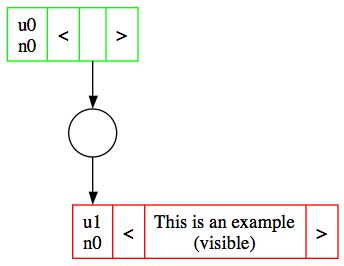
\includegraphics[width=2.0in]{tree1zz.jpg}
\caption{Tree after inserting "This is an example.\label{fig:tree0}"}
\end{figure}

\subsubsection{Inserting a substring}
Next suppose that the user 1 decided to insert the word "interesting"
before "example."  This can not be handled as an extension of the node
$u1/n0$.  As above, this will actually be inserted one character at a time
in most cases (unless the user cut and pastes the word from some other
document into the buffer). Since this is an insertion in the middle of a node,
the system will generate a tree-edit operation which adds a new node $u1/n1$
containing the character $i$ and attaches that node at position 11 of the
parent node $u1/n0$.  As the user continues to type the word "interesting"
the successive characters are added to the node $u1/n1$ as $u1$ is the owner
of the node and the insertions are at the end of the node. The result
is a new node containing the entire word "interesting" attached at position
11 of its parent. The tree in the left side of Figure \ref{fig:tree11}
shows the resulting edit-tree.



\subsection{Creating conflicts in collaborative editing}
Next, suppose user $u3$ 
simultaneously inserts the adjective "illustrative "
before the word "example" in their own
local copies and that both users broadcast their edits to their peers, which
includes user 2 who is just watching the other two edit.  
In a high latency environment (or in a setting where the user's are queueing 
their edits before sending them out), user 2 would create its own tree
but with a different node attached at position 11 of the $u1/n0$. This tree
is shown in the right side of Figure \ref{fig:tree11}. Again, if user 3
is typing the word character by character then the first character will generate
the node $u3/n0$ containing only one character.

Lets look at this more closely.
We assume at a given point in time all users share the same edit-tree as shown 
in Figure \ref{fig:tree0}. Then they all have the string view
\[
\alpha_i= \text{"This is an example."}
\]
Now, if user 1 applies the string operation
\begin{verbatim}
  insert(11,"interesting ")
\end{verbatim}
this will be translated into the following edit-tree operation
\begin{verbatim}
  treeinsert(u1/n0:19,11,u1/n1,"interesting ")
\end{verbatim}
which states that the new node $u1/n1$ containing the text "interesting"
should be added as a child of the node $u1/n0$ at position 11 out of 19. Applying
this operation results in the edit-tree in the left side of Figure \ref{fig:tree11}
and in the following edit-string view
\[
 <_0^0 <^1_0 
 \text{This is an }<^1_1 
 \text{interesting}
>^1_1  \text{example.} >^1_0 >_0^0
\]
Similarly for user 3 who applies the string operation
\begin{verbatim}
  insert(11,"illustrative ")
\end{verbatim}
which is translated into the following edit-tree operation
\begin{verbatim}
  treeinsert(u1/n0:19,11,u3/n0,"illustrative ")
\end{verbatim}
resulting in the following edit-string corresponding to the edit-tree
in the right side of Fig \ref{fig:tree11}
\[
 <_0^0 <_0^1 
 \text{This is an} <^3_0 
 \text{illustrative}
>^3_0  \text{example.} >_0^1 >_0^0
\]


\begin{figure}[h]
\vspace{\baselineskip}
  \hspace{\fill}\rule{\linewidth}{.7pt}\hspace{\fill}
  \vspace{\baselineskip}

\centering
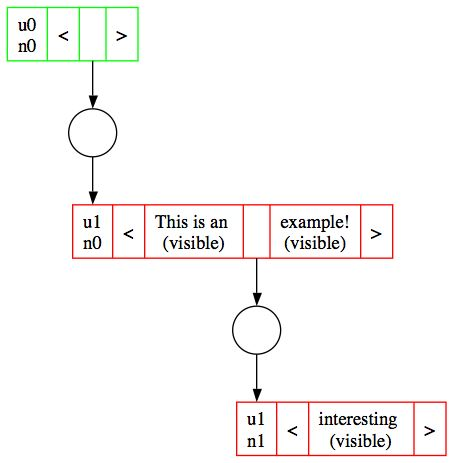
\includegraphics[width=2in]{tree11.jpg}
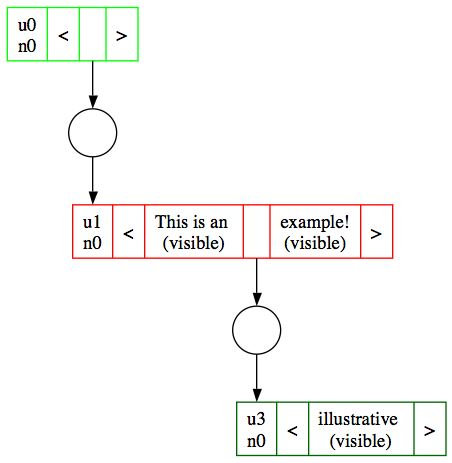
\includegraphics[width=2in]{tree12.jpg}
\caption{Tree $T_1$ on the left after user 1 inserts "interesting ,
and tree $T_3$ on the right after user 3 inserts "illustrative ".\label{fig:tree11}}

\centering
\vskip 0.3in
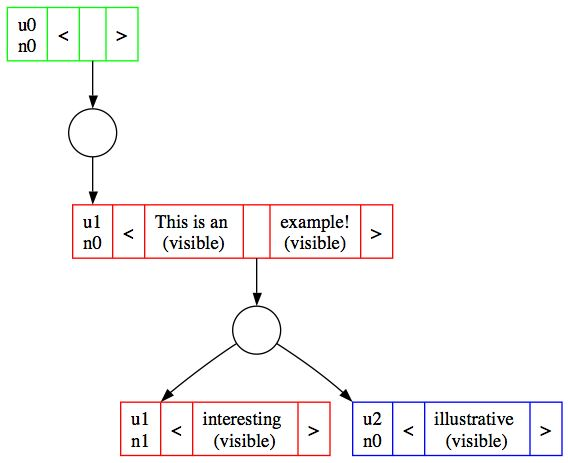
\includegraphics[width=3in]{tree13.jpg}
\caption{Trees after inserting both "interesting " and "illustrative ".\label{fig:tree13}}


\vspace{\baselineskip}%
  \hspace{\fill}\rule{\linewidth}{.7pt}\hspace{\fill}%
\vspace{\baselineskip}%
\end{figure}

\subsection{Handling conflicts in collaborative editing}
When user $u_2$ receives these tree-edit operations there will be an
apparent conflict. Both $u1$ and $u2$ want to insert a string at position
$11$ of $u1/n0$.  

The MSET approach is to allow multiple users to insert at
the same position, but to order the insertions by user id, and to disallow
the same user from inserting multiple times at the same position in the edit-tree.
Thus, if there are $k$ users, then there could be up to $k$ children nodes
attached at any particular position of an edit-tree node.

In this case, conflict resolution results in the tree in Figure
\ref{fig:tree13} where $u1/n0$ has two children nodes attached at position $11$,
the node $u1/n1$ is on the left and $u3/n0$ on the right as $u1<u3$.
This strategy for handling conflicts guarantees that all users will have
the same edit tree, no matter which order they apply the edit-tree operations.

In the case where the new nodes were created one character at a time, rather
than using cut/paste to insert the words, the conflict would occur with two
nodes that each contain a single character and will be resolved in the same
way.  Also, the users doing the editing $u1$ and $u3$ will receiving the
conflicting edit operation and will create the correspond nodes and modify
their string views without changing the relative cursor position. Thus as they
continue typing their edits will be used to extend their nodes and the
same tree will result as if they had used cut/paste to insert the words.


\subsection{Deletion as hiding}

We handle deletion by marking characters stored in the nodes of the edit-tree 
to be either "visible" or "hidden."  Deleting a substring in the standard string
view of the document is translated into an edit-tree operation where the
corresponding characters are marked as "hidden."  Any user can "hide" any
characters, even in nodes they do not own, but no user can "unhide" characters.
Once they are deleted they cannot be made visible again. Rather one must
reinsert the characters. (We will discuss an algorithm for relaxing this
restriction later).

Continuing with our example, supposer user 1 receives user 3's edits
and so has the string view
\[
\text{This is an interesting illustrative example.}
\]
and deletes the word "interesting". This
results in
\[
\text{This is an illustrative example.}
\]
The deletion gets transformed into a "hide" operation which results in the
tree in Figure \ref{fig:tree14} which has the following edit-string representation:
\[
 <^0_0 <^1_0 
 \text{This is an} 
   <^1_1 \text{\sout{interesting}} >^1_1
  <^3_0 \text{illustrative} >^3_0
  \text{example.} >^1_0 >^0_0
\]

\begin{figure}[h]
\vspace{\baselineskip}
  \hspace{\fill}\rule{\linewidth}{.7pt}\hspace{\fill}
  \vspace{\baselineskip}

\centering
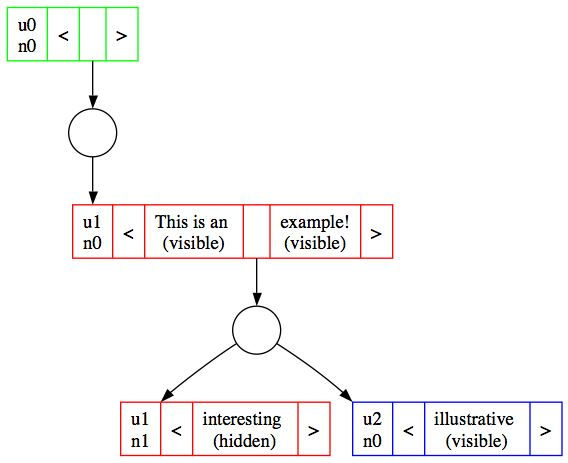
\includegraphics[width=2in]{tree14.jpg}
\caption{Deletion as hiding. Observe that the node $u1/n1$ has the
label "hidden"  beneath its text, whereas the other nodes have "visible".
This indicates that all text in that node is "hidden". \label{fig:tree14}}

\vspace{\baselineskip}%
  \hspace{\fill}\rule{\linewidth}{.7pt}\hspace{\fill}%
\vspace{\baselineskip}%
\end{figure}

\subsection{Inserting into a tree with hidden characters}
Suppose now that user 2 has received all of these edits
and wishes to insert the word ``easy''
into the place where ``interested'' had just been deleted by user 1.
This would result in the following string:
\[
\text{This is an easy illustrative example.}
\]
The point we want to make here is that there are several places that the new node
$X = <^2_0 \text{easy} >^2_0$ could be inserted in the tree
which would place it between "an" and "illustrative" in the string view.
Several possibilities are shown below and their corresponding edit-trees
are snown in Figures \ref{fig:tree14a} and \ref{fig:tree14b}

If the insertion had been done by user 1 rather than user 2, then there
is another option, which would be to modify the edit-tree by appending
"easy" to the text in $u1/n1$ right after the hidden text "interesting".
This is shown in Figure \ref{fig:tree14d}.
\begin{itemize}
\item {\bf leftmost insertion}
The first possibility is to insert the new node directly before the
first character (visible or hidden) after the insertion point. This
is in fact would the current implementation of MSET would select
for this particular example,
but any of these operations could be used.
\[
 <^0_0 <^1_0 
 \text{This is an} 
   <^1_1 <^2_0 \text{easy} >^2_0 \text{\sout{interesting}} >^1_1
  <^3_0 \text{illustrative} >^3_0
  \text{example.} >^1_0 >^0_0
\]
\item {\bf rightmost insertion}
The next is to insert it as far to the right as possible in
the edit-tree.
\[
 <^0_0 \;<^1_0 
 \text{This is an} 
   \;<^1_1 \text{\sout{interesting}} >^1_1\;
  <^3_0 \;<^2_0 \text{easy} >^2_0 \;\text{illustrative} >^3_0\;
  \text{example.} >^1_0\; >^0_0
\]
\item {\bf insertion in a hidden string}
Yet another possibility is to insert it somewhere else (anywhere) in the node $u1/n1$
which contains only hidden text.
\[
 <^0_0 <^1_0 
 \text{This is an} 
   <^1_1 \text{\sout{interesting}} <^2_0 \text{easy} >^2_0>^1_1
  <^3_0 \text{illustrative} >^3_0
  \text{example.} >^1_0 >^0_0
\]
\item {\bf insertion as a child of $u1/n0$}
The final possibility is to insert it as another node at the same level
as $u1/n1$ and $u3/n0$, which would result in
\[
 <^0_0 <^1_0 
 \text{This is an} 
   <^1_1 \text{\sout{interesting}}>^1_1
   <^2_0 \text{easy} >^2_0
   <^3_0 \text{illustrative} >^3_0
 \text{example.} >^1_0 >^0_0
\]
\end{itemize}
These are all the possibly ways in which the edit observed in the string view
could be obtained by a valid edit on the edit-tree.

\subsection{Insertion points depend on the user}
Note, the set of such possible edits depends on which user was doing the
editing. Indeed, 
if the word "easy" had been inserted by user 1 instead of user 2,
then another possiblility
would arise. 

{\bf extension of a hidden node owned by the user}
User 1 could just extend the node $u1/n1$
and not create a new node at all, as shown below and in Figure \ref{fig:tree14d}.
\[
 <^0_0 <^1_0 
 \text{This is an} 
   <^1_1 \text{\sout{interesting}easy}>^1_1
  <^3_0 \text{illustrative} >^3_0
  \text{example.} >^1_0 >^0_0
\]


\begin{figure}[h]
\vspace{\baselineskip}
  \hspace{\fill}\rule{\linewidth}{.7pt}\hspace{\fill}
  \vspace{\baselineskip}

\centering
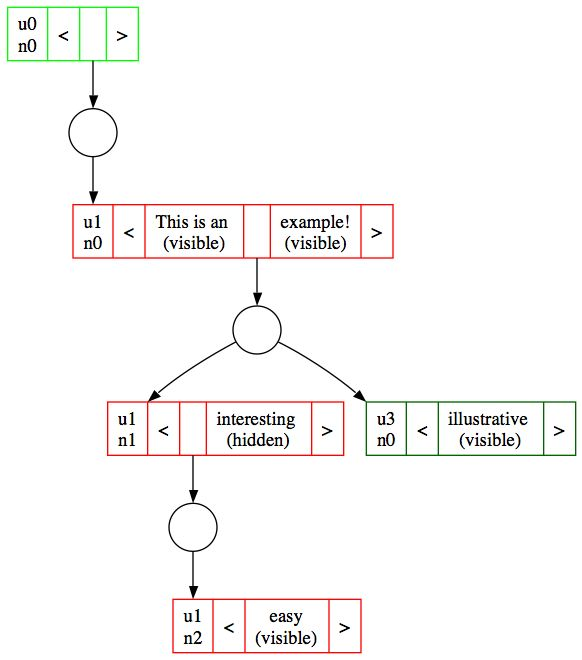
\includegraphics[width=2in]{tree14b.jpg}
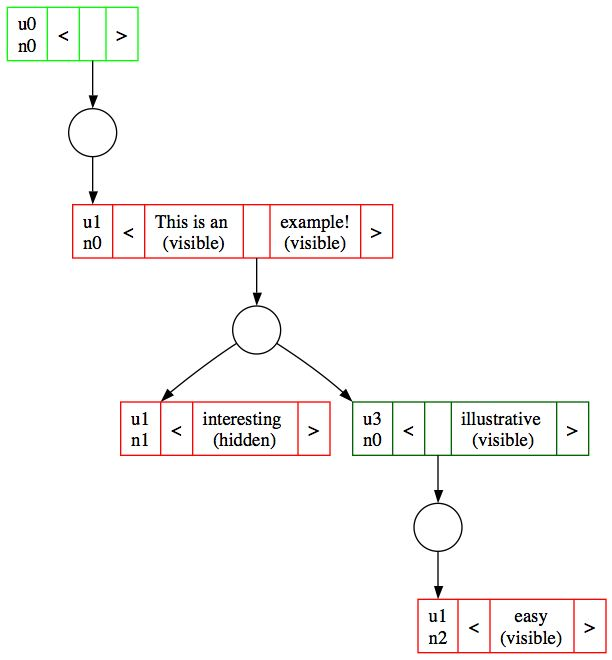
\includegraphics[width=2in]{tree14a.jpg}
\caption{Two ways for user 1 to insert ``easy '' 
between ``an '' and ``illustrative ''. The MSET algorithm
would generate the tree on the left. \label{fig:tree14a}}

\vspace{\baselineskip}%
  \hspace{\fill}\rule{\linewidth}{.7pt}\hspace{\fill}%
\vspace{\baselineskip}%
\end{figure}


\begin{figure}[h]


\centering
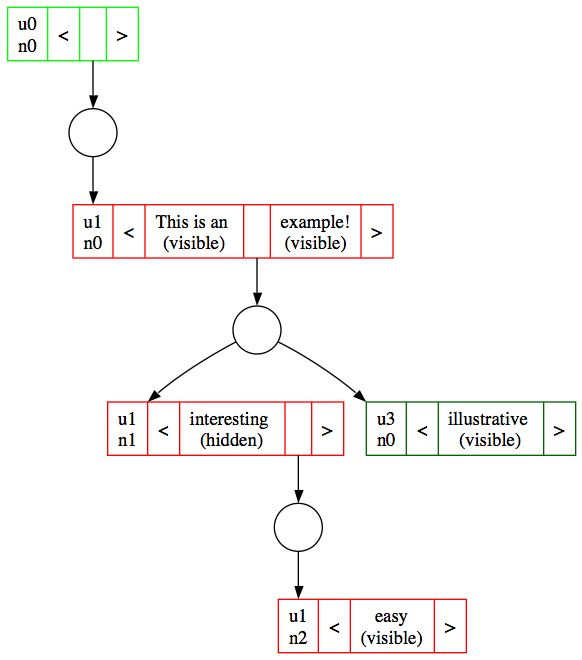
\includegraphics[width=2in]{tree14c.jpg}
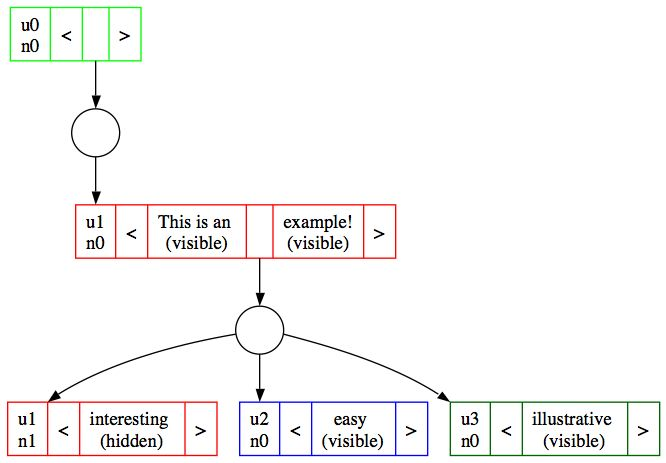
\includegraphics[width=2in]{tree14e.jpg}

\caption{Two more ways for a user to insert ``easy '' 
between ``an '' and ``illustrative ''.\label{fig:tree14b}}


\vspace{\baselineskip}
  \hspace{\fill}\rule{\linewidth}{.7pt}\hspace{\fill}
  \vspace{\baselineskip}

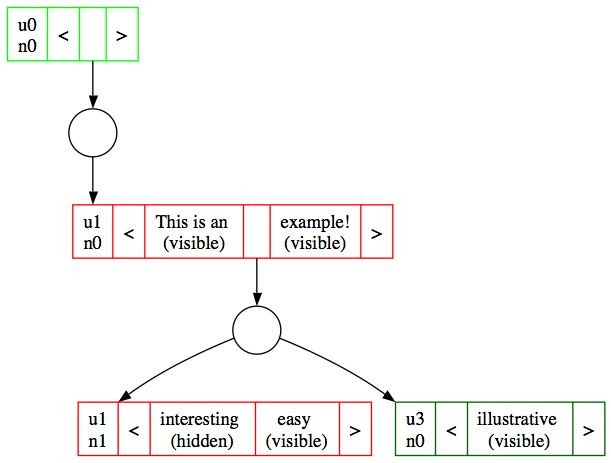
\includegraphics[width=3in]{tree14d.jpg}

\caption{An additional option if the insert was by user 1.
Observe that the text ``easy'' appears with the label ``visible''
in the node $u1/n1$ following the pre-existing hidden text
``interesting'' This is a valid edit operation only if the user
that created the insertion operation is the owner of the node
being extended. In this case, both are $u1$. \label{fig:tree14d}}

\vspace{\baselineskip}%
  \hspace{\fill}\rule{\linewidth}{.7pt}\hspace{\fill}%
\vspace{\baselineskip}%
\end{figure}

Note that we could not insert node $X$ directly before the $<^1_1$ marker
as that would violate the property of edit-trees that all children of a
node attached at the same point must be ordered by their userid and there
must be at most one node for each user. In this case, user 1 would have two
nodes inserted at position 11 of $u1/n0$ which is not allows.

\subsection{General features revealed by the example}
This extended example demonstrates the fundamental ideas behind the MSET
approach. Each user $u_i$ represents the shared document as an edit-tree $T_i$
which has two different views: the standard view $\alpha_i = f(T_i)$ which
is the string of visible characters in $T_i$, and an edit-string view
$\beta_i = g(T_i)$ which contains the hidden characters as well as the
start and end markers for the nodes. The user can insert and delete anywhere
in the standard view, but can only mark characters as "hidden" in the
edit-string view and can only insert at selected places in the edit-string
view. The string operations are converted to edit-tree operations which are
broadcast to all of the peers in the collaborative editing group. Those users
apply the remote operations they receive in any order they choose, provided only
that they wait for the target node of an operation to be created before the'
operation is applied.

We will describe the algorithm in more detail below and we will show that it
can be implemented in such a way that each local and remote edit operation
can be performed in time $O(k\log(N))$ where $k$ is the number of characters
in the operation and $N$ is the size of the edit-string.



\section{The unoptimized distributed model for edit trees}
% Here we describe the model at the level of nodes without worrying about an efficient
% implementation. We can describe the late joining protocol and the central server vs
% distributed server model.

As mentioned in the introduction the MSET model is based on the notion that 
each user maintains an edit tree as the underlying model of the textarea in
which they are editing. In this section, we describe an algorithm for 
collaboratively editing the edit-trees directly. In a later section we will show
how to extend this to an editor of edit-strings as well as strings in
the standard view. Then we'll show how to implement these algorithms
efficiently. In this section, we assume that the users are only interested in editing
the trees directly.

\subsection{Definition of an edit-tree}
We make the following assumptions about the structure of the edit-trees:
\begin{itemize}
\item Each user has a unique ID from some totally ordered set $U$ of userids 
and the nodes of the edit-tree 
are labelled with the userid and an integer which uniquely identifies
that node among all created by that user.
\item Each node contains a sequence of one or more characters.
\item Each character has a boolean visibility property which is set
to false when the character is "deleted". 
\item The nodes can have children nodes.
Each such child is attached at a particular position in the string.
\item Multiple nodes can attach to the same position, but no two nodes that are owned by the 
same user can be attached at the same position. The nodes that are attached at
a given position are ordered by userid. 
\item The root of the tree is owned by the
superuser "u0". This user does not own any other nodes and does not insert any
text into the root node. 
\end{itemize}

\subsection{Valid edit operations on an edit-tree}
We place restrictions on the type of edits that can be performed
on an edit tree. Indeed, there are only three actions a user $u$ can take
when editing their copy of the shared edit tree. We will indicate nodes 
of the edit-tree being edited by
the notation $u/n$ where $u$ is the user who created the node and $n$ is an
integer uniquely identifying this node among all nodes created by the user.

There are three operations a user $u$ can perform on a node and the operations
that can be performed depend on the user. To simplify the presentation, we only consider operations that handle a single character at a time.

Let $v/m$ denote the $m$th node created by user $v$.
User $v$ will be able to append characters to the end of $v/m$, so 
we will sometimes futher indicate that node by $(v/m:p)$
where $p>0$ is the number of characters in $v/m$. This allows us to
distinguish between different versions of a single node.

Let $u$ be the user performing one of the following tree tree edit operations
on the target node {\tt v/m:p} to create a new node {\tt u/n:q}.
\begin{itemize}
\item ${\tt treeextend}(v/m:p,\alpha)\;\;\text{if u=v}$ \newline
First, user $u$ can extend the text in the node $v/m$
provided it is the owner (that is $v=u$). It extends the node by appending
some character $\alpha$ to the location $p$ at the end of the node,
Note however, that users can not modify
the text in any node that they do not own and can not change any of the text
once it has been put into the node.
\item ${\tt treeinsert}(v/m:p,q,u/n:1,\alpha) \;\; \text{if $q\le p$}$
\newline
Second, user $u$ can insert a new node $u/n$ containing a character $\alpha$
at any position $q\le p$ of the node, 
$v/m$ provided
they have not already inserted a node there. If one or more nodes have already been inserted there, then they must be arranged in order of the userid and the new node is inserted into this sorted sequence by userid.
\item ${\tt treehide}(v/m:p,q)  \;\; \text{if $q\le p$}$\newline
Third, user $u$ can set the visibility of a character at position $q < p$
in  $v/m:p$ to false.
When characters are initially added to a node they have visibilty true, but once
set to false, the visibilty must remain false. 
\end{itemize}
For all of these operations, we say that the node $(v/m:p)$ is the target of the edit operation and the node that is created, either $(v/m:p+1)$ for an extension or $(u/n:1)$ for a new node, is the result.  

We use these definitions to define a partial order on edit operations $\tau\prec\tau'$ where $\tau$ directly preceds $\tau'$ if the result of $\tau$ is the target of $\tau'$, and we let $\prec$ be the transitive closure of that relation.  Then $\prec$ is a partial order on the set of all possible edit operations on a tree. We say that two operations $\tau$ and $\tau'$ are independent if neither precedes the other, that is 
\[
\left (\tau\not\prec\tau'\right ) \wedge  \left ( \tau'\not\prec\tau \right )
\]
Observe that operations performed simultaneously by two clients on their own local edit trees are clearly independent from each other.

Given these definitions and rules we see that a group of distributed users can easily edit a 
shared tree by keeping their own representation of the tree and broadcasting
their edits to their peers. Observe that these edit operations commute in
the following sense. The only place where two user's could have a editing
conflict is when they both want to insert a string of characters at a particular
position $q$ in some node $v/m:p$, but in this case their insertions are always
ordered by userid and this resolves the conflict. No matter which order the
operations are applied the same tree results. This is phrased more formally
in the following lemma:

\begin{lemma}
Let $T=T_0$ be any edit-tree and let $\tau_0,\tau_2,\ldots,\tau_{n-1}$
be a sequence of valid edit operations on $T$ as described above.
This yields a sequence of edit trees $T_0,\ldots,T_n$. Let 
$\tau'_0,\ldots,\tau'_{n-1}$ be any reordering of this sequence of operations
which is topologically sorted with respect to $\prec$, that is
with the property that if $i<j$ then either $\tau'_i\prec\tau'_j$ or
$\tau'_i$ and $\tau'_j$ are independent. Let $S_0=T_0$ and $S_{i+1} = \tau'_i(S_i)$.
Under these assumptions, the corresponding sequence of trees
$S_1,\ldots,S_n$ is well-defined and $S_n=T_n$.
\end{lemma}

\begin{proof}
First, the sequence $S_{i}=\sigma_i(S_{i-1})$ is well-defined because we have
stipulated that the target of each $\sigma_i$ must exist in $S_{i-1}$ so the
operator can be applied. To see that the two resulting trees are equivalent
we simply observe that the extend operations for a node $v/m:p$ must appear
in the same order in the $\sigma_i$ as the $\tau_i$ and since they effect only
the node $v/m$ the node $v/m$ will contain the same string in both $S_n$ and $T_n$.
The insert operations for a given node $v/m$ on the other hand can appear
in any order and their effect will be to add children to positions $q$
of the final node. When multiple insertions attach to the same position, they
will be ordered by user id. Since they are inserted into an ordered list,
the order in which they are inserted doesn't matter.
\end{proof}

\subsection{Distributed editing of edit trees}
In the previous subsection we showed that any valid ordering for a sequence
of tree edit operations will yield the same final result. We can use that
observation to define a distributed algorithm which converges provided only
that a fair network property is assumed.

The model is that we will have a set $G$ of clients $C=C_1,\ldots,C=C_n$
all starting with the empty tree. Each client $C_i$ has a unique userid $u_i$,
a local copy $T_i$ of the shared edit tree,
a list $Q_i$ of edit operations that other users have applied but which it
has not yet processed, and
and a map $H_i$ from nodeids $v/m$ to nodes of the edit tree or to sets of tree-edit operations using a union type. If the tree $T_i$ contains a node $A$ with nodeid $v/m:p$ then $H_i(v/m:p)=A$, otherwise $H_i(v/m:p)$ is a list $S$ of tree-edit operations taken from $Q_i$ whose target is $v/m:p$.

We assume that the clients observe the following protocol. 
In particular user $u_i$ can do the following:
\begin{itemize}
\item Perform a valid operation $\tau$ on their local copy of the tree to
produce a new (or extended) node $n$ with nodeid $u/n:q$,
after which they set $H_i(u/n:q)$ to $n$ and they also add $\tau$ to $Q_j$ for
all $j\ne i$.
\item Take an operation $\tau$ from $Q_i$. If the target of $\tau$ is
in $T_i$ then $\tau$ is applied to the tree to produce a node $v/m:p$
and the tree-edit operations in $H_i(v/m:p)$, if any, are inserted back into $Q_i$
 and $H_i(v/m:p)$ is set to $n$.
\end{itemize}
Note, this model can easily be extended to allows for late joiners by having users
maintain a history list $Q'_i$ of all operations they have applied to their tree. 

Any user $k$ who joins the group notifies all users it has joined and waits for confirmation from all users. Once this is obtained, it 
requests some client $C_j$ to forward its current history list $Q'_k$ and its current queue, 
$Q_k$ into its own edit queue $Q_i$.
This can be an incremental copy at user $j$'s leisure depending
on the workload.  This may require user $k$ to check each new operation
it receives to make sure that it has not already been received and processed,
but this is not too expensive.

\begin{lemma}
Let $G$ denote a collaborative editing session as described
above and assume that all clients $C_1,\ldots,C_n$ follow the protocol above
for a certain period of time and then stop. Once all queues $Q_i$ have been
emptied and all operations processed, all users will have the same edit
trees, that is if $T_i$ is the final edit tree of $C_i$, then $T_1=T_2=\ldots=T_n$.
\end{lemma}

\begin{proof}
This follows easily from the previous lemma where we let $\tau_1,\ldots,\tau_m$
denote the sequence of operations performed by user $1$ and let 
$\sigma_1,\ldots,\sigma_m$ denote the operations performed by user $i$. Then
these are clearly valid rearrangements of each other and by the previous
lemma the resulting trees are the same.
\end{proof}

\section{From edit-trees to an optimally efficient collaborative editor}
In this section we will define the MSET data type $M$ which simultaneously maintains
four views of an editing session
\begin{itemize}
\item $M.S$ - the standard string view of a text-editing session, a sequence of characters from a character set $\Sigma$
\item $M.R$ - a revisions view which is a sequence of characters which each have a visibility attribute (visible or hidden), this is similar to the tracking-changes view of modern text editors
\item $M.E$ - an edit-string view which is a sequence of attributed characters and marker symbols (start markers $<^u_n$ and end markers $>^u_n$)
\item $M.T$ - an edit tree
\end{itemize}
The three string views are all views of the edit tree $M.T$ obtained by traversing the tree in infix order and recording the characters and or symbols of the specified type.

Our approach will be demonstrate that insertions and deletions on $M.S$ can be
transformed efficiently (in time $O(\log(N))$ where $N$ is the size of $M.T$) into
tree-edit operations on $M.T$.  We will also show that the three tree-edit operations
on $M.T$ can be performed in time $O(\log(N))$ and that for each tree-edit operation $\tau$ we can calculate the corresponding string edit operations on $M.S$, $M.R$, and $M.E$ in time $O(\log(N))$.  If we assume that we have a system which will maintain the string views of $M.S$, $M.R$, and $M.E$ then this approach allows us to accept string-edit operations on $M.S$ from the user, use them to construct a corresponding tree-edit operation $\tau$ and then broadcast that $\tau$ to all other users.  Moreover, for each tree-edit operation $\tau$ generated locally or received from a remote user, the corresponding string-edit operations $\sigma_S, \sigma_R, \sigma_E$ can be efficiently generated and sent to the systems which are maintaining those views.

In this section, we define the MSET data type and prove that its operations can be performed in time $O(\log(N))$ where $N$ is the size of $M.T$.

The data type $M$ is created in constant time by a constructure $newMSET(u)$ that creates an empty tree $M.T$ and empty strings $M.S, M.R, M.E$ for the user $u$.

The data type $M$ allows the following operations:
\begin{itemize}
\item $M.treeextend(v/m:p,\alpha)$ - lookup the node with nodeid v/n:p and extend it by adding the character $\alpha$ at position $p$, update the lists $M.S$, $M.R$, and $M.E$ as well.
\item $M.treehide(v/m:p,q)$ - set the visibility to false for the element at position $q$ of the node with id $v/m:p$
\item $M.treeinsert(v/m:p,q,u/n,\alpha)$ - create a new node with id $u/n:1$ containing the single visible character $/alpha$ and insert that new node at offset $q$ in the node with id $v/m:p$.
\item $M.converttotreeop(\sigma)$- returns a tree-edit operation $\tau$ on $M.T$ that corresponds to the string edit operation $\sigma$ on $M.S$
\item $M.converttostringop(\tau,X)$ - return the string edit operation (and insertion or deletion) for the string $M.X$ which correspond to applying the tree edit operation $\tau$ on $M.T$
\end{itemize}
The three tree operations also a triple of string operations that can be applied to
the views $M.S$, $M.R$, and $M.E$ so they will agree with the modified $M.T$.
We will provide algorithms for all five of these operations and prove that their complexity is $O(\log(N))$.
\subsection{implementation of characters and markers}
We assume all visible characters come from an alphabet $\Sigma$
and we expand that alphabet to $\Sigma^*$ by including all start and endmarkers.
The elements in the lists and the tree will be represented by a tuple that contains links to the nodes and also links to an indexing object $M.I$ which will allow one to rapidly calculate the position of the element in the lists (i.e. the number of elements of type $S$, $R$, or $E$ to the left of the element) and also allows us to rapidly find the $k$th element of each of the three lists.

We represent the elements of these strings by tuple containing
\begin{itemize}
\item {\tt symbol} - a character or start marker or end marker 
\item {\tt visible} - a boolean (used to distinguish visible from hidden characters)
\item {\tt node} - a link to the node of the edit tree containing this element
\item {\tt nodeid} - a convenience field giving the id $v/m:p$ of the node
\item {\tt offset} - the offset of the element in the node, which is either a non-negative integer or is {\tt start} or {\tt end} for the markers.
\item {\tt indexTree} - a link to the index tree node corresponding to this element
\end{itemize}

\subsection{Implementation of the lists $M.S$, $M.R$, and $M.E$}
The three lists will be represented by doubly linked lists together with an index
tree that provides $O(\log(N))$ access to the elements by their offset in the three lists. 

The index tree $M.I$ can be implemented as a balanced binary tree whose leaves are the elements in $M.T$ and which stores at each internal node, a triple containing the number of elements of type $S,R,E$ in the subtree below that node. Clearly such a structure can support insertion of elements in time $O(\log(N))$ by inserting and rebalancing (e.g. with red/black trees) and then updating the element count triples in the modified nodes. This structure allows us to implement the following  operations so they can be computed in time $O(\log(N))$ where we assume we have already calculated the node and offset for $e$ in $M.T$
\begin{itemize}
\item {\tt M.insertBefore(e,f)} - insert element $e$ before element $f$ in $M.E$ and reflect those changes in $M.R$ (resp. $M.S$) as well so that they remain the subsequence of $M.E$ consisting of non-marker (resp. visible) elements.
\item {\tt M.insertAfter(e,f)} - similar to the above, but insert $e$ after $f$
\item {\tt M.insertAtStart(e)} - insert $e$ at the beginning of $M.E$.
\item {\tt M.hide(e)} - this sets the visibility of $e$ to $false$ and removes $e$ from $M.S$, updating the indexTree $M.I$ in the process.
\end{itemize}

\subsection{Implementation of the tree $M.T$}
The edit tree will be implemented as a rooted set of linked nodes.
The nodes contain a sequence of elements as well as the links to children nodes
Each node has the following fields:
\begin{itemize}
\item {\tt userid} - the unique id for the user who created this node
\item {\tt count} - the number of nodes created by that user before this one
\item {\tt elt[]} - an array list of elements
\item {\tt insertionSet[]} - an array list of insertion sets providing access to the children nodes inserted at each position in the node
\end{itemize}
Each {\tt insertionSet} maintains a sequence of nodes, ordered by userid where
each element can be accessed in $O(\log(N))$ time (actually $O(\log(U))$ time where $U$ is the number of users active in creating $M.T$ but that is less than or equal to the number of nodes in $M.T$).


\subsection{Efficient implementation of $M.converttotreeop(\sigma)$}
This function takes a string operation $\sigma$ on $M.S$ and converts it into
an equivalent tree operation 
$\tau$ on $M.T$ such that
$\Gamma_S(\tau(M.T)) = \sigma(\Gamma(M.T))$.

There are two possibilities for $\sigma$, either it is an insertion of a character $\alpha$ at offset $k$ in $M.S$ or it is the deletion of the character $\alpha$ at position $k$ in $M.S$.  

\paragraph {{\tt delete($k$)}} 
Lets handle the deletion case first as it is easiest. The first step is to lookup the element $e$ at position $k$ in $M.S$. This can be done in time $O(\log(N))$.
We can then use $e$ to lookup the node $n$ and offset $q$ of $e$ in that node.
This takes time $O(1)$ the node and offset are fields of $e$. Finally, we lookup the
nodeid $v/m$ and length $p$ of $n$ and generate the operation $treehide(v/m:p,q)$. This operation takes time $O(\log(N))$. In pseudocode, we have
\begin{verbatim}
delete(k)
  e = M.I.lookupS(k);
  v/m:p = e.nodeid;  q = e.offset
  return treehide(v/m:p,q)
\end{verbatim}

Next lets handle the case where $\sigma$ is the insertion of the character $c$
at offset $k$ of the string $M.S$.  There are five cases to consider:

\subsubsection{Case 1: inserting at the beginning of a string: $k=0$}
In this case, we are to insert $c$ at the beginning of the string.
The first step is to look up the first element $e$ of $M.R$ in time $O(\log(N))$.
This is the first non-marker element in $M.T$. Using $e$ we lookup the
nodeit $v/m:p$ of the node containing $e$ and we observe that $e$ must be at position 0 in this node (as it is the first non-marker element in $M.E$. Therefore
we generate the tree operation $treeinsert(v/m/p,0,u/n,c)$. This takes total time $O(\log(N))$.
\begin{verbatim}
insertcase1(k,c)
  e = M.I.lookupR(0);  n = e.node; v/m:p = e.nodeID
  return treeinsert(v/m:p,0,u/n,c)
\end{verbatim}

\subsubsection{Case 2: inserting at the end of a string}
This case is similar. We start by looking up the last element $e$ in the revisions view $M.R$ which is also the last non-marker element in $M.E$. This takes time $O(\log(N))$, we can also look up the nodeid $v/m:p$ of the node in time $O(1)$.  There are
two cases, if $u=v$ then we can generate a tree extend operation
$treeextend(v/m:p,c)$ and otherwise we generate a insert operation
$treeinsert(v/m:p,p,u/n,c)$.
\begin{verbatim}
insertcase2(k,c)
  e = M.I.lookupR(0);  n = e.node; v/m:p = e.nodeID
  if u==v then return treeextend(v/m:p,c)
              else  return treeinsert(v/m:p,p,u/n,c)
\end{verbatim}

\subsubsection{Case 3: inserting in the middle of the string}
in this case we can lookup the elements $e$ and $f$ on either side of the insertion point $k$ in $M.S$. This takes time $O(\log(N))$.  We can look up the offsets $k_1$ of $e$ in $M.E$ and $k_2$ of $f$ in $M.E$ and look at the elements between $e$ and $f$ in $M.E$. There are three subcases to consider here depending on the type of the element $g$ that follows $e$ in $M.E$.

\subsubsection{Case 3a: $g$ is a non-marker element}
In this case, $g$ is either $f$ or a hidden character, but in any case, we can insert $\alpha$ between $e$ and $g$. So in time $O(1)$ we lookup the nodeid $v/m$ and
offset $q$ of $g$ and generate the tree edit operation 
$treeinsert(v/m:p,q,u/n:1,c)$

\subsubsection{Case 3b: $g$ is an end marker}
In this case, we look up the node id $v/m$ of $e$ as before and if $u=v$
then we can extend the node with $treeextend(v/m:p,c)$ whereas if $u\ne v$
then we use a standard insertion $treeinsert(v/m:p,q,u/n,c)$.

\subsubsection{Case 3c: $g$ is a start marker}
in this case, all of the nodes between $e$ and $f$ must be start markers,
so we can insert $\alpha$ directly before $f$.  Look up the nodeid $v/m:p$ of $f$
in $O(1)$ time and generate $treeinsert(v/m:p,0,u/n,\alpha)$

\begin{verbatim}
insertcase3(k,c)
  e = M.I.lookupS(k-1); f = M.I.lookupS(k);
  v/m:p = e.nodeid; 
  g = e.nextE /* get element after e in M.E */
  if not g.isMarker
    treeinsert(g.nodeID,g.offset,u/n:1,c)
  else if g.isStartMarker
    treeinsert(f.nodeid,0,u/n,c);
  else if g.isEndMarker & u==v
    treeextend(v/m:p,c)
  else
    treeinsert(v/m:p,p,u/n,c)
\end{verbatim}
We have consider all of the possible cases and hence this demonstrates that 
$M.converttotreeop(\sigma)$ can be implemented with complexity $O(\log(N))$.




\subsection{implementing $treehide(v/m:p,q)$}
The first step is to lookup, in time $O(\log(N))$ the node $n$ with id $v/m:p$
and to then look up the element $e$ at offset $q$ in time $O(1)$. 
To hide $e$ we simply set the visible value to $false$.

Once we've found the element $e$ to be hidden, we can
calculate the position $k_S$ of the element in $M.S$ in time $O(\log(N))$
and generate the string op $delete(k_S)$. The same process can be applied to
$M.R$ and $M.E$ to generate $delete(k_R)$ and $delete(k_E)$, which should
change the view for the character to indicate it has been "deleted".

\begin{verbatim}
treehide(v/m:p,q)
  n = M.lookupNode(v/m:p);
  e = n.elt[q]
  M.I.hide(e)
  /* return view op to update M.S, M.R, M.E */
  return delete(e.listOffset)
\end{verbatim}


\subsection{applying $treeextend(v/m:p,c)$ on $M.T$}
Again, we first lookup the node $n$ with id $v/m:p$ and then lookup the 
end marker element $f$ of $n$. We can then create a new element $e$
using $alpha$ and the node id $v/m:p$. We can then insert $e$ into
$M.E$ by inserting it before the end marker $f$ of $e$ and then adjust 
the indexing trees for $M.S$, $M.R$, and $M.E$.

Using this node $n$, we can calculate the number
of elements $(k_s,k_r,k_e$ of each type (visible, non-maker, any) that appear before $e$ in
the three lists (in time $O(\log(N))$ and generate the string ops $stringinsert(k_X,\alpha)$ for $X in \{s,r,e\}$.

\begin{verbatim}
treeextend(v/m:p,c)
  n = M.lookupNode(v/m:p);
  f = n.endmarker
  e = Element.new(c,n)
  M.I.insertBefore(e,f)
  return insertBefore(f.listOffsets,c)
\end{verbatim}

\subsection{applying $treeinsert(v/m:p,q,u/n,\alpha)$ to $M.T$}
This is the trickiest tree edit operation and requires several cases..

\subsubsection{converting $treeinsert(v/m:p,q,u/n,\alpha)$ to a string op}
Again, we lookup the node $n$ with id $v/m:p$ and the element $e$ at position $q+1$ if $q<p$ or the end position $e$ if $q=p$. 


\subsection{Main Theorem}

\section{MSET-based Collaborative Editing}








\section{The unoptimized model for edit trees with a edit-string view}
We are really interested in collaborative editing of strings, not trees, so the
question arises as to how we can convert string edit operations of the user
into tree edit operations on the user's model, and how we can convert tree edit
operations from the user's peers into string edit operations on the user's string.

As a first step, observe that there is a one-to-one correspondence between
edit-strings as defined above and edit-trees, thus our distributed algorithm
for edit-trees provides a distributed algorithm for edit-strings where we
assume that the clients $C_i$ each maintain a edit-string $S_i$ and perform valid
edit-string operations on $S_i$. These operations can be transformed directly
into valid tree operations which can be broadcast to the peers above. 

This raises the question of which string edit operations are valid operations,
in the sense that they correspond to the valid tree-edit operations described
in the previous section.  Clearly any non-marker node can be "deleted" by setting
its visibility property to "hidden."  The insertion operations are a little
trickier, but its not hard to show that the following operations are precisely
those which correspond to valid-tree operations. 

We describe the valid edit-string insertion operations as insertions
between two symbols $d_i$ and $d_{i+1}$ in the edit-string, where the $d_i$
is one of the following:
\begin{itemize}
\item  a character, $c_i$, either visible or hidden,
\item  a start marker $<^v_m$ or
\item an end marker $>^v_m$
\end{itemize}
Based on this categorizations, there are nine possibilites for inserting a character between two adjacent elements in an edit string. In each case we could either enter a single character $\alpha$ or a node $<^u_n \alpha >^u_n$ containing that character. The next lemma considers all of those possibilities and specifies which ones correspond to legal operations on an edit tree.

Let $u$ denote the user performing
the operation and let $n$ be the next available block id for user $u$, so if
the user inserts a new block containing the character $\alpha$, it will be inserted
as $<^u_n \alpha >^u_n$.  Let $c_i$ and $c_j$ denote non-marker characters in
a block $v/m$ 
which could be either visible or hidden or one of each and let
 $v$ and $w$ be users different from $u$ and each other.

\begin{lemma} Notation as above. There are 9 cases for inserting a character or a node containing a character into an edit string between two elements $c_i$ and $c_{i+1}$ in an edit string within the scope of a node $v/m$. The following cases specify which possibilites correspond to valid operations on the edit tree and which do not. If a case is not listed, then it is not valid. 
\begin{eqnarray}
c_i\;\;\;\;\; c_{i+1} &\rightarrow& c_i <^u_n \alpha >^u_n c_{i+1} \label{eq:ins1}\\
c_i\;\; >^w_r &\rightarrow& \left\{ 
  \begin{array}{l l}
      c_i \alpha >^w_r &  {\rm if}\; u=w  \label{eq:ins2a}\\
      c_i <^u_n \alpha >^u_n >^w_r &  {\rm if} \; u \ne w 
  \end{array}  \right . \label{eq:ins2b}\\
c_i \;\;<^w_r &\rightarrow& \left\{ 
\begin{array}{l l}
c_i <^u_n \alpha >^u_n <^w_r & {\rm if}\; u<w  \label{eq:ins3a}\\
{\rm INVALID} & {\rm if} u \ge w \label{eq:ins3b}\\
\end{array}
\right . \label{eq:ins3}\\
>^v_m \;\;c_{i+1} &\rightarrow& 
 \left\{ 
  \begin{array}{l l}
    >^v_m  <^u_n \alpha >^u_n c_{i+1} & {\rm if} \; v<u \label{eq:ins4a}\\
   {\rm INVALID} & if v \ge u \label{eq:ins4b}\\
  \end{array} \right .\label{eq:ins4}\\
>^v_m \;\;>^w_r &\rightarrow& 
  \left\{
    \begin{array}{l l}
      >^v_m \alpha >^w_r &{\rm if}\; u=w \label{eq:ins5a} \\
      >^v_m <^u_n \alpha >^u_n >^w_r & {\rm if} \; (v<u)  \&  (v \ne w)  \label{eq:ins5b} \\
     {\rm INVALID} & {\rm (v > u) \& (v \ne w)} \label{eq:ins5c}
    \end{array}\right . \label{eq:ins5} \\
>^v_m \;\;<^w_r &\rightarrow & 
\left \{
\begin{array}{l l}
 >^v_m <^u_n \alpha >^u_n <^w_r & {\rm if} \; v<u<w  \label{eq:ins6a}\\
{\rm INVALID} & {\rm otherwise}  \label{eq:ins6b}
\end{array} \right . \label{eq:ins6}\\
<^v_m \;\;c_0 &\rightarrow& <^v_m  <^u_n \alpha >^u_n c_0\label{eq:ins7}\\
<^v_m \;\;>^w_r &\rightarrow& 
\left \{
\begin{array}{l l}
<^v_m <^u_n \alpha >^u_n >^w_r & {\rm if} \; v=w=0, r=m=0 \label{eq:ins8a}\\
{\rm INVALID} & {\rm otherwise} \label{eq:ins8b} \\
\end{array} \right . \label{eq:ins8}\\
<^v_m \;\;<^w_r &\rightarrow&
\left \{
\begin{array}{l l}
 <^v_m <^u_n \alpha >^u_n <^w_r & {\rm if} \; u<w  \label{eq:ins9a}\\
{\rm INVALID} & {\rm otherwise}  \label{eq:ins9b}\\
\end{array} \right . \label{eq:ins9}
\end{eqnarray}
\end{lemma}

\begin{proof}
Case (1): Note that user $u$ can always insert a new node between any two non-marker
characters (Eq. \ref{eq:ins1}), using operation $treeinsert(v/m:p,q,u/n,\alpha)$ but
since the position is not at the end of the node a straight insertion of $\alpha$ is not allowed.

Cases (2) and (5): User $u$ can always insert a string
directly into the end of a node that it owns via $treeextend(v/m:p,\alpha)$
 (Eqs. \ref{eq:ins2a}, \ref{eq:ins5a}) 
but the user can also insert a node at that position if they want $treeinsert(u/n:p,p,u/n,\alpha)$ if no node has been inserted there yet
 (Eq. \ref{eq:ins2b}). If another node has already been inserted at the
last position by user $v$ then user $u$ can only insert a node there if $v<u$.

Case (3):
A node $u/n$ can be inserted as the first node at an insertion point if the current
first node in the insertion point $w/m$ satisfies $u<w$.

Case (4):
A node $u/n$ can be placed at the end of an insertion point where the last node in the insertion is $v/m$ if and only if $v<u$.

Case (6):
A node $u/n$ can be inserted between two nodes $v/m$ and $w/r$ in an insertion point if and only if $v<u<w$.

Case (7): a node $u/n$ can always be placed at position 0 of a node $v/m$ provided nothing has yet been inserted there.

Case (8): 
The only case where a start symbol is immediately followed by an end symbol
if the root case $<^0_0>^0_0$ and in this case, user 0 is the root and does not insert any elements itself, so the only thing that can be inserted is a node, i.e. not a character (Eqs. \ref{eq:ins8a}, \ref{eq:ins8b} ).

Case (9): a node $u/n$ can be inserted at the position 0 of a node $v/m$ which already has some nodes inserted there if and only if the first node inserted a position 0, $w/r$ satisfies $u<w$.

\end{proof}



For now, we observe that if a edit-string view only allows the insertions
as shown above for user $u$, then each such insertion corresponds to a valid
edit-tree operation and hence the collaborative editing protocol in the previous
section for edit-trees can be naturally extended to edit-strings.  The converse
is also true, every valid edit-tree operation corresponds to one of the 9 valid cases above.


The following
lemma states the convergence property for this distributed algorithm.


\begin{lemma}
Let $G$ denote a set of clients $\{C_1,\ldots,C_n\}$
that are running the collaborative
editing protocol for their local copies of edit-strings $S_i$
starting with empty strings.
Suppose they perform some number of valid
edit operations and then stop editing and process all operations in their queues.
Then, 
we will have $S_1=S_2=\ldots=S_n$.
\end{lemma}



\section{The unoptimized model for edit trees with a standard-string view}

This model is only slightly more complicated than the previous case of
collaborative editing of edit-strings.  In this case, each client maintains three
views of the editing process: the standard view of the string currently being edits,
the "tracking changes" view which shows both the visible and "deleted" characters (with a different font of the deleted characters), and the edit-string view which
has characters (both visible and hidden with appropriate attributes for each type)
and markers (both start and end). 

Our first observation is that each character in the standard view corresponds
to a uniquely defined visible character in the tracking-changes view, and
each character in the tracking-changes view corresponds to a non-marker character in the edit-string view. So we are really maintaining one list and two nested sublists of that list.

There are two operations we allow on the standard view:
\begin{itemize}
\item ${\tt insert}(p,\alpha)$ - insert the character $\alpha$ 
at offset $p$ in the string
\item ${\tt remove}(p,\alpha)$ - remove the character $\alpha$ at offest $p$
which has the effect of changing the attribute of that character from visible to hidden.
\end{itemize}

If $T$ is a edit-tree and $S = \Gamma(T)$ denotes the standard string view
of that tree, then we want to show that for each string operation $\sigma$
on $S$ there is a corresponding valid operation $\tau$
on the edit-tree, such that 
\[
\Gamma(\tau(T)) = \sigma(\Gamma(T))
\]
This will allow us to convert string operations into edit-tree operations which
can then be broadcast to all users as in the previous section. There can be more than one possible $\tau$ operation that satisfies this property (and often there are many), but all we need is the existence of at least one such operation. At this point, we don't worry about the computation complexity of calculating the edit-tree operation corresponding to a string operation, that will be the subject of the next section.

The remove operation is easily transformed into a edit-tree hide operation which 
simply sets the visibility attribute of the corresponding character to "hidden''.

The insert operation is a bit trickier mainly because, as we have
seen in the example at the beginning of this paper,
a single insert position in
the standard view could correspond to many different insert positions in the 
edit-tree, not all of them legal.

We now describe how to find one such $\tau$ and in the next section we present a data type in which that $\tau$ can always be constructed in time $O(\log(N))$.


There are four basic insert operations on the string $S=\Gamma(T)$ in the standard view to consider.
\begin{itemize}
\item inserting into an empty string
\item inserting at the beginning of the string
\item inserting at the end of the string
\item inserting somewhere in the middle of the string 
\end{itemize}
The first case is easily handled as it results in the following operation on the 
edit-string $\gamma$:
\[
<^0_0\;>^0_0 \;\; \rightarrow \;\;<^0_0 <^u_0 \alpha >^u_0 >^0_0
\]
The second is a little trickier. We need to find the first non-marker character $d_k$
in the full-edit string and observe that the previous character must be a start
marker $<^v_m$ so we can insert the new node $u/n$ containing $\alpha$ between those
two points, where $n$ is the number of nodes owned by $u$ in $T$ and observe
that inserting a new node 
\[
<^u_n \alpha >^u_n
\]
between a start marker and a non-marker character is always valid.

The third case of inserting at the end of the standard view is similar. One
must find the last non-marker character (visible or hidden) $d_k$ in the
edit-string $\gamma$ and observe that $d_{k+1}$ must be an end marker
$>^v_m$ thus we can insert $u/n$ between $d_k$ and $d_{k+1}$ as a valid
edit-string operation.

The last case is when we are inserting between two characters $c_i$ and $c{_i+1}$
in the standard view $S = \Gamma(T)$. Let $d_j$ denote the visible non-marker
character corresponding to $c_i$ in the edit-string $T$ and let
$d_k$ denote the next non-marker character. So $d_j$ and $d_k$ are non-marker
characters, all the symbols between them are marker symbols, $d_j$ is
visible, and $d_k$ could be visible or hidden. There are three subcases:
\begin{itemize} 
\item $d_{j+1}$ is a non-marker character, i.e. $d_j$ and $d_k$ are adjacent. 
In this case, inserting
the node $u/n$ between them is always valid.
\item $d_{j+1}$ is an end marker $>^v_m$, again in this case inserting $u/n$
between $d_j$ and $d_{j+1}$ will be a valid insert operation.
\item $d_{j+1}$ is a start-marker. In this case all of the symbols between
$d_j$ and $d_k$ must be start markers, so $d_{k-1} = <^v_m$ is a start marker
and inserting between that symbol and the non-marker character that follows
is a valid operation.
\end{itemize}
In each of these three cases, we get a edit-string operation $\tau$ that
corresponds to inserting $\alpha$ between $c_i$ and $c_{i+1}$. The arguments
above have proven the following lemma.


\begin{lemma}
Let $T$ be a edit-tree and let $S=\Gamma(T)$ be its standard string view, then
the algorithm described above constructs a valid edit-tree operation $\tau$
on $T$ for each valid edit operation $\sigma$ on the string $S=\Gamma(T)$,
we have
\[
\sigma(\Gamma(T)) = \Gamma(\tau(T))
\]
\end{lemma}


We can now define a
collaborative editing algorithm where the user $u$ presents 
a standard view of a
string $S^u_i$ representing the effect of $i$ editing operations.
The user can then either insert or delete a character from that string
and broadcast the corresponding edit-tree operation to all peers.
Likewise, edit-tree operations that are received from peers can be applied to
the tree results in a modifed string $S^u_{i+1}$. Since the edit operations commute as long as they are independent, the order in which they are applied doesn't matter!
This proves the following theorem.

\begin{theorem}
The full-edit-tree collaborative editing algorithm as described above
is convergent, that is, if all users start with the same tree $T_i=T$ and
all perform a set of editing operations as described above, then after all
editing has stopped and all messages have been received and processed, all clients
will have processed the same number $n$ of edit operations (some local and
some remote) and all will have the same edit tree stored in their local copy
$T_i$.
\end{theorem}


So far we have described a relatively simple collaborative editing algorithm and
proved that it is correct . We have not shown however how
to implement it efficiently. A naive implementation would require time $O(N)$ for
each step, where $N$ is the size of the edit-string. (This would happen
for example if the edit-tree is comb-shaped which would require time $O(N)$
to traverse from the root to the farthest leaf.)

We will show in the 
next section, that this time can be reduced to $O(k\log(N))$ where $k$ is the
size of the operation (i.e. number of characters inserted or deleted) and
$N$ is the size of the edit-string (i.e. the number of characters inserted
and/or deleted by the collaborative users).


\section{Optimizing the model}
% Here we describe the subnode implementation with red-black trees and the initial and
% final subnodes for each node. We prove that the operations are optimally efficient.

We have shown that edit-trees can be used to implement a collaborative editor
which allows the user to immediately apply local edits and which has the convergence
property.  The model as presented in the previous section becomes unacceptably slow ($O(N)$ for each insert and delete) as the size of the tree grows if we use a naive data structure to represent the three lists and the edit tree.  

In this section, we show how to optimize this model by creating a more complex representation which allows
the string to tree and tree to string conversions on edit operations to be computed
in time $O(\log(N))$ where $N$ is the size of the edit tree.

In particular, the MSET algorithm will maintain the edit tree $T$ as described above,
but will also maintain an auxiliary data structure $M$ that allows it to rapidly
compute the node position in the edit tree corresponding to an element (i.e. a visible or hidden character or a start or end marker) in any one
of three string views, and vice versa. The three string views are
\begin{itemize}
\item $M.S$: the "standard" list of all visible characters
\item $M.R$: the "tracking changes" list of all visible and hidden characters which shows all of the revision of the document,
\item $M.E$: the "edit-string" list of all edit-string characters which faithfully represents the edit-tree by showing all visible and hidden characters and all markers (both
start markers and end markers)
\end{itemize}
We will show that these three lists can be implemented in such a way as to be able
to calculate the $k$th element of each list (e.g. M.E[k]) in time $O(\log(N))$ where $N$ is the size of the edit-tree. Moreover, given an element $e$ its position in any one of these lists can also be computed in time $O(\log(N))$ using $M.pos(e,L)$ where $L$ is one of $S,R,E$.  In case, $e$ doesn't appear in a list of type $L$ (e.g. a marker character in the $S$ or $R$ list) we can also evaluate $M.posBefore(e,L)$ and $M.posAfter(e,L)$ which return the index of the element e in the list of the specified type or the index of the first element $f$ of that type which appears before (or after) that element in the edit-string. This can be useful when we want to compute the first character that appears before a start marker for example. We will show that this can also be computed in time $O(\log(N))$. 

More precisely, we will describe a new data type, which we call the Monotone Shared Edit Tree datatype which maintains 3 simultaneous representations of a user's edit-session corresponding to the standard, tracking changes, and edit-string views discussed above. This data type allows users to perform five different operations.
Two operations on the standard view (insert or delete a character) and three operations
on the edit-tree view (extend a node, insert a node into a node, or hide a character in a node). The operations are notated as shown below:
\begin{itemize}
\item $insert(k,\alpha)$ - insert character $\alpha$ at offset $k$ in the standard view and generate a corresponding edit-tree transformation $\tau$
\item $delete(k,\alpha)$ - delete the character $\alpha$ at offset $k$ in the standard view and generate a corresponding edit-tree transformation $\tau$
\item ${\tt treeextend}(v/m:p,\alpha)$ - extend the node $v/m:p$ by appending
a character $\alpha$ to the location $p$ at the end of the node and generate
the corresponding string transformation $\sigma$.
\item ${\tt treeinsert}(v/m:p,q,u/n,\alpha) $ -
 insert a new node $u/n$ containing the character $\alpha$
at position $q\le p$ in $v/m:p$ and generate
the corresponding string transformation $\sigma$.
\item ${\tt treehide}(v/m:p,q)$ - set
 the visibility of the character at position $q < p$
in  $v/m:p$ to false and generate
the corresponding string transformation $\sigma$. 
\end{itemize}
We will show that each of these operations can be computed in time $O(\log(N))$ where $N$ is the size of the edit string.

We will apply this to a collaborative editing system where each client
performs standard string edit-operations received locally from its user
and also performs tree-edit operations received from remote users.
For local edit operations, it converts them to edit-tree transformation, applies them 
to the local edit-tree and broadcasts the transformation to all peers. For remote edit-tree transformation, it applies them to its local tree, calculates the corresponding string operation and applies that locally to the standard view.


In the rest of this section we will formally define the MSET data type and prove that each of the local and remote operations can be performed in worst case time $O(\log(N))$

The MSET data type $M$ is implemented by maintaining the three list views using a three balanced binary trees where each in each tree node contains the number of elements of the specified type in its subtree. Looking up an element by its index and type can be performed in time $(O(\log(N))$.
Insertion of a new element between two elements of the list can be performed by adding a node to all three trees and rebalancing if necessary while maintaining the counts of number of leaves beneath each node. This can be done in $O(\log(N))$ time as well. In addition to maintaining these three lists, the system also maintains an edit tree representation and stores, for each element, the node and offset in which it appears in the tree. The key idea is to implement the edit tree in such a way that each local and remote editing operation can be performed in time $O(\log(N))$ while preserving the relationship between the three views and the edit tree. 

We will represent each of the characters (visible, hidden, or marker) uniquely as an
element of type Atom.  With this approach, the lists $S$ and $T$ are sublists of $E$.

An Atom element will have the following fields:
\begin{itemize}
\item $nodepos$ this takes values of the form $(u/i/p)$ which specify the position $p$ of the atom in the $ith$ node created by user $u$.
\item $visible$ - this boolean value is true if the character is visible, false otherwise. It is false for the marker symbols and characters are "deleted" by setting this field to false.
\item $character$ - this is the character at that position which is either a character typed in by the user, or is a start marker $<^u_i$ or an end marker $>^u_i$.
\end{itemize}
Optionally, we can add a "node" field which gives a direct link to the corresponding node in the edit tree. This reduces look time from $O(\log(N))$ to $O(1)$ but
doesn't improve the asypmptotic performance so we will skip it in this version.

Each node $N$ in the edit tree will be represented by the following components:
\begin{itemize}
\item $N.user$ which is the user who created this node
\item $N.nodecount$ which is the number of nodes created by the user before this one
\item $N.atom$ which is an arraylist where $N.atom[i]$ will be a link to the $i$th atom in the node, where $i$ is a position consisting of a non-negative integer.
\item $N.start$ the atom holding the start marker for this node
\item $N.end$ the atom holding the end marker for this node
\item $N.insertionSet$ where $N.insertionSet[k]$ is a balanced binary tree map $S$ of the nodes inserted at position $k$ in the node.
Recall that nodes are inserted at each insertion point in a list ordered by their
userids. $S(u)$ gives the node $n$ owned by user $u$ and inserted at that position, if it exists; or gives a pair of nodes $n1,n2$ on either side of the position where a node owned by user $u$ should be inserted. We need this data structure to be able to rapidly process remote insertions with conflicts at the same position in a node. 
\end{itemize}
The insertion set is the key innovation which is needed to obtain logarithmic performance. It is required when processing an insertion operation at a conflict point, i.e. a point where several other users have simultaneously inserted an element. Since one could have $O(N)$ possible users, and these collision nodes are all ordered by user id, one needs to be able to lookup the correct position in time $O(\log(N))$ and hence some sort of balanced tree data structure is required.

We now present the MSET algorithm for each of the five possible edit operations: local insertion, local deletion, remote extension of a node, remote insertion of a node, and remote hiding of a character in a node.


\subsection{Insertion of a character in standard string view}

In this section we show how implement the local insert operation 
\[
insert(k,\alpha)
\]
for user $u$ assuming that it has already created $n$ nodes and that $\alpha$ has length $d=1$. This will get converted into one of the following two operations:
\begin{itemize}
\item ${\tt treeextend}(v/m:p,\alpha)$ 
\item ${\tt treeinsert}(v/m:p,q,u/n:1,\alpha) $
\end{itemize}
and will create a new element $e$ that gets inserted into each of the three lists
$M.S$, $M.R$, and $M.E$.

We must determine which type of transform is appropriate and to find the node $v/m:p$ and possibly the offset $q$ 
in time $O(\log(N))$.
Once these are calculated, they can be applied in time $O(\log(N))$ by using
a balanced binary tree search to find the node with id $v/m:p$ and the extension
of that node or the insertion of a new node can then be completed in time $O(d)$.


Lets look at the simple cases first, that is where we are inserting at the
beginning or the end of the string. 

In the insertion is at the beginning ($k=0$), we need to find the first non-marker (hidden or visible) element $A=M.R[0]$ in the "tracking changes" view which will be at offset 0 in a node $v/m:p$. This takes time $O(\log(N))$.
From $A$ we can lookup the node id $v/m:p$ in constant time so the operation gets transformed into 
$tree_insert(v/m:p,0,u/n:d,\alpha)$. The new node $e$ corresponding to the character can then be created and inserted into $M.S$, $M.R$, and $M.E$ in
$O(\log(N))$ time.
 
This case of inserting at the end is similar, except that we need to find the last element $A$ in the tracking changes view. 

This leaves the cases involving inserting into position $k$ in the middle of the string.
The first step is to look up the atoms $A_1=M.S[k]$ and $A_2=M.S[k+1]$ on either side of
the insertion point in the standard view and we then calculate the offset $k'$ of $A_1$ and $k''$ of $A_2$ of these atoms in the edit-string view and
the element $A' = M.E[k'+1]$ following $A_1$. This takes
$O(\log(N))$ time. There are three cases to consider.

\subsubsection{Case 1: the element $A'$ in the edit-string is a non-marker character}
In this case, we can lookup the node $v/m:p$ and offset $q$ of $A'$ in constant time and insert the new node containing $\alpha$ directly before  $A'$ with
$treeinsert(v/m:p,q,u/n,\alpha)$. We then need to create the element $e$ corresponding to this character and insert it into $M.S$, $M.R$, and $M.T$.
Since we already have the non-marker element $A'$ we can insert it into those
lists in time $O(1)$ or $O(\log(N))$ if it is a hidden character and we need to find the nearest  non-hidden character in $M.S$.

\subsubsection{Case 2: the element $A'$ is an end marker for node $v/m:p$}
In this case, if $u=v$ then we can extend the node using $\alpha$ and otherwise
we insert a new node containing $\alpha$ at the end of $v/m:p$. The element
corresponding to $\alpha$ can be inserted into $M.S$, $M.R$, and $M.T$ as in case 1.

\subsubsection{Case 3: the element $A'$ is start marker}
In this case, all of the elements between $A_1$ and $A_2$ must be start markers
and so we can insert $\alpha$ right before $A_2$.  So we look up the node id $v/m:p$ of $A_2$ and insert a new node at position $0$ of $v/m:p$ we also create a new element for the character $\alpha$ and insert it before $A_2$.

These arguments show that any insert operation can be converted to an edit tree operation in time $O(\log(N))$.



\subsection{Deletion in the standard string view}
Consider now the problem of deleting the character $\alpha$
 at position $k$ of the string.
In this case,
we find the node $v/m:p$ and offset $q$ corresponding to the character $\alpha$ to be deleted by looking up $M.S[k]$ in time $O(\log(N))$
and we simply set the visibility flag to "hidden" for that character.

\subsection{Extension transformation on the edit-tree}
This is quite easy. We lookup the node to extend in time $O(\log(N))$
extend it in time $O(1)$, look up the corresponding element in time $O(1)$,
and calculate its position in the standard string view $M.S$ in time $O(\log(N))$
then delete it from the string view in time $O(\log(N))$.

\subsection{Tree-insertion in the edit-tree view.}
Lets now assume we have received a tree-insertion operation $\tau$
to insert a new node $u/n$ containing a text string $\alpha$  
at position $q$ 
in the node $v/m$

Our first step is to lookup the node $N$ with id $v/m$ in time $O(\log(N))$
and then to access the insertionSet $S=N.insertionSet[q]$ at offset $q$
and then to create a new node $N'$ with id $u/n$ containing $\alpha$.
This insertion set is between two elements $A'$ and $A''$ of the edit-string.
There are a few cases.

If $S$ is empty, then we simply insert $N'$ into $S$ and insert the element
corresponding to $\alpha$ into the appropriate positions in $M.S$, $M.T$, and $M.E$. This can all be done in time $O(\log(N))$.

If $S$ is not empty, then it holds a sequence of nodes by different users and none of those nodes are owned by $u$.  Since it is a balanced tree we can lookup the position where $N'$ needs to be inserted in time $O(\log(N))$. There are three
cases. First, if $N'$ needs to be inserted at the beginning of $S$, then 
it will be inserted directly after $A$. Likewise, if $N'$ needs to be inserted at the
end of $S$, then it will be inserted directly before $A'$.  These take time $O(\log(N))$ to insert in the lists and rebalance the trees.

The only remaining case, is that $N'$ must be inserted between consecutive two nodes $N_1$
and $N_2$ in S. We then lookup the end position element $B$ of $N_1$ and insert $N'$ directly after $B$. This again takes time $O(/log(N))$ to find $N_1$ and $N_2$
and time $O(/log(N))$ to insert the element corresponding to the inserted character $\alpha$ into the three lists and rebalance the trees. 


\subsection{Tree-hide operation in the edit-tree view}
The problem of processing a tree-hide operation $\tau$ to hide 
a character at position $q$ in node $v/m:p$ is easier.

We lookup the node with id $v/m:p$ in time $O(\log(N))$ and
then we find the element at position $q$ in the node
and set the attribute to $hidden$ in time $O(1)$. Then we remove the
node from the $M.S$ list and rebalance the tree.

\subsection{Main theorem}
We have therefore proved 

\begin{theorem}
The MSET data type processes each of the two standard string operations (insert and delete) and
the three edit-tree operations (treeextend, treeinsert, treehide) in time $O(\log(N))$ where $N$ is the size of the edit-tree before the operation is performed.
\end{theorem}

This in turn proves that the MSET-based collaborative editing system is convergent and optimally efficient.

\begin{corollary}
The MSET data type can be used to implement a convergent, collaborative editing system where each local operation can be performed in time $O(\log(N))$ and each remote tree-edit operation can be performed in time $O(\log(N))$ where $N$ is the side of the current edit tree, which is proportional to the total number of elements that have been inserted into the local edit string (whether or not they have later been deleted).
\end{corollary}

%\section{Extensions and Applications}
%
%\subsection{Collabed} 
%In 2007, we implemented the MSET algorithm and used it to create several plugin for standard 

%%%%  Work getting parts of the rest of this into the main article
%\newpage
%\section{Details of a Pratical M}
%In practice, we don't use node positions of size 1 but rather use subnodes
%of size 1 or more that consist of sequences of characters that all share the
%same attribute (e.g. hidden or visible). This complicates the algorithms
%as deletion requires one to split subnodes which are then reinserted into
%the data structure $M$, but it greatly decreases the speed of the algorithm
%(not asymptotically of course). Moreover, we don't introduce explicit
%start or end marker nodes of size zero unless they are needed, which only
%occurs if there is an insertion at the beginning or at the end of a node.
%
%Also, discuss algorithms for preferring extensions rather than
%inserts where possible.
%
%%% KGG needs to change data references to characters to maintain consistency
%
%\subsection{Introducing Subnodes}
%$Subnode$: A reference to a segment of an MSET node's sequence of characters that
%share the same set of attributes and does $not$ have any insertions.
%
%Bold Assertion: We can't minimize node creation by merging node data (e.g.
%creating strings from characters) without introducing subnodes. To do so would
%restrict the use of attributes.
%%lookup times to degrade to O(N) vs O(log(N)).
%
%%% I'm not sure that our auxiliary data structure $M$ is to be viewed as three
%%% doubly linked list as described in section 6.1 Efficient implementation of M
%%% but rather as described in this section as one large doubly linked list of 
%%% subnodes and N=(number of nodes) smaller linked list.
%
%Thus far we have discussed the MSET data structure as a tree of nodes containing
%an arraylist of attributed characters and an arraylist of insertion positions.
%Now we are going to introduce subnodes that place the markup
%of raw MSET data on a separate plane, but more importantly, 
%enables the grouping of sequences of characters with identical attributes.
%That is, the raw MSET data (full string view)
%is still stored in MSET nodes as it did before, but now, attributes are stored
%in a linked list of subnodes for optimum maintenance. This also enables faster
%seek times at the expense of extra meta data.
%
%%Another significant reason for including subnodes is to optimize the MSET node
%%space complexity by introducing node extensions. 
%
%$Node Extension$: Append newly inserted data $k$ at the end of an existing node's
%data $N(c)$ instead of creating a new node when the following rules are upheld:
%
%%% rule 1) is greatly simplified here because it is not handling full view
%%% and standard view differences. Mainly, the most frequent case of hitting the
%%% backspace key as we type prevents real extensions unless we check for it.
%\begin{verbatim}
%  1) The new data is being inserted at the end of a node.
%  2) Both the new insertion and the node that is to be extended is
%     owned by the same user.
%\end{verbatim}
%
%These rules are required to maintain MSET's convergence mechanism, uniquely
%ordered and identifiable edits. With insertions being identified by u/n/p,
%allowing extensions of any other form would corrupt the MSET.
%
%
%
%\subsection{Balanced Lookup Trees}
%The core principle of an MSET is that all edits are permanent, one directional,
%monotone. This principle is to be extended to attributes as well. To do so more
%clearly we introduce balanced subnode trees that are provide the means for
%fast conversions between node positions and string offsets (M.lookupNodePos, 
%M.lookupStrPos) and also maintains the attribute set of raw MSET data.
%
%As described before, we are just balancing an indexed MSET based inserts and
%attributed node segments to achieve O(log(N)) lookup complexity when going back
%and forth between node view and string view. The idea is to have all the subnodes
%make up the leaves of the balanced binary tree. Thus each parent node would
%pivot on the sum of its children sizes as depicted in \label{fig:rbtree14e}.
%
%\begin{figure}
%\centering
%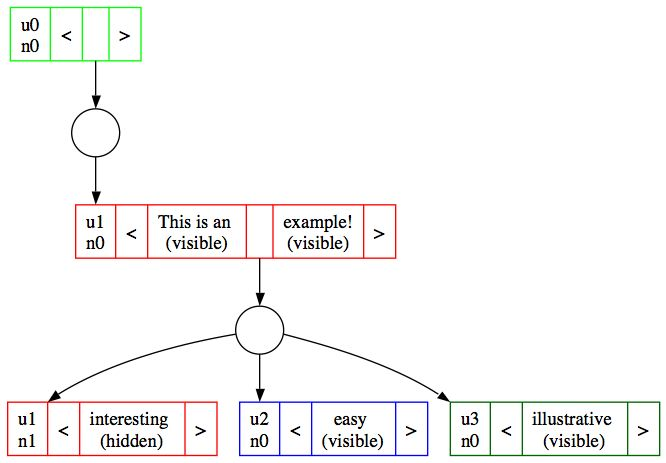
\includegraphics[width=2.4in]{tree14e.jpg}
%%\includegraphics[width=2.4in]{tree14e-rb.png}
%
%\caption{Natural Node View -VS- Balanced Binary Subnode View.\label{fig:rbtree14e}}
%
%\vspace{\baselineskip}
%  \hspace{\fill}\rule{\linewidth}{.7pt}\hspace{\fill}
%  \vspace{\baselineskip}
%\end{figure}
%
%A global balanced tree $GT$ sits a top a linked list of all subnodes and each
%MSET node has a local balanced tree $LT$ that sits a top a linked list of its
%subnodes. 
%
%
%\newpage
%\section{Extensions}
%\subsection{Allowing more general attributes}
%One simple extension to this model allows it to support general text attributes
%(e.g. font-style, text-color, etc.) which can be changed multiple times by
%the users while preserving the convergence property.
%
%The key idea is to associate with each character both an attribute set and a
%priority value. The priority value consists of a positive integer $k$ and a userid $u$
%indicating the author of the last change and the priority of that change. 
%When a user $u$ changes an attribute, the generate a tree edit operation which
%increments the priority $k$ and sets the author to $u$. When a user receives
%a remote attribute change operation with priority $(k',u')$ it compares that
%priority with the current priority $(k,u)$ and only applies the attribute
%change if $(k',u') > (k,u)$, that is if $(k'>k) \vee (k=k')\wedge(u'>u)$.
%Note that unless we use an unbounded representation (e.g. java.math.BigInteger)
%for the priority $k$
%that there will be a maximum priority $k_max$ after which no additional
%changes to the attribute set will be allowed. This is probably not a practical
%problem if one uses at least 16 bits for the priority.
%
%This extension works well with the subnode optimization as one can associate
%an attribute to an entire subnode and hence change the attributes of the text
%in a subnode in time $O(1)$
%
%
%\subsection{Late Joining}
%Late joining can be implemented by allowing a late joiner to ask another
%user to send its history and queue to the late joiner.  The late joiner
%keeps track of which nodes it has received from each user and can tell
%when it is up to date. This assumes that the users generate node id's
%sequentially.  To optimize this we can structure the history mechanism
%as ordered list of users, and for each user a vector of edit operations
%and a vector of "holes" which are operations that have been generated but
%have not yet been received.  In addition, each node it will contain an
%ordered list of extension operations.
%
%\subsection{Adding backchannel communication}
%We have found it useful to increase awareness by adding video, audio, or
%text-based communication to the editing session. This is not an algorithmic
%extension to the editor, but in practice most user's do have the ability to
%add an audio or visual connection.  For large groups that are not collocated,
%a shared text-based chat window would also work, possibly with speech generation
%to keep the visual space free.
%
%\subsection{Managing the queues of incoming and outgoing edit operations}
%The MSET model can easily accommodate the introduction of queues of incoming
%and outgoing tree-edit operations and we have found it helpful to allow the
%user to turn on an off the queueing of incoming and/or outgoing edit operations.
%Queueing the incoming edit operations
%is similar to locking a document in that a user's edit session is not
%interrupted by remote edit operations but remote users are able to continue 
%editing and can even edit the user's text as it is being generated. This
%is particularly useful when the user is performing a repeating macro on
%the edit window (e.g. applying some emacs-macro to every line of a file).
%It is also useful when entering an "undo" session as we describe in the next subsection.
%
%Queueing both incoming and outgoing operations is helpful if the user wants to
%work on a part of the document and doesn't want any other user to be able to
%edit the section until it is complete.  This is helpful for example, when
%co-editing a Java program if the user is refactoring a procedure. Other users
%can continue to edit and compile the code without these changes being visible
%until they are complete.
%
%Disconnection from the network can be handled transparently by turning on the
%queueing of incoming and outgoing edit-operations. When the network is rejoined
%the user perform a late joining request to another user (ideally a high bandwidth)
%user, where that user sends its history and queues to the reconnecting user
%in reverse order (i.e. most recent first). The reconnecting user filters out
%those operations that have already been processed (and are in the 
%node lookup table)
%
%\subsection{Undo}
%
%It is a good idea to enter an "undo" mode in which all incoming edit operations
%are queued while the undo process is active as this will allow the user to
%revert the system to the state they want before continuing.
%
%\subsubsection{Global Undo}
%The simplest form of "undo" which reverses the most recent non-undo edit operation
%is easy to implement.  One keeps a history of the string-based edit operations
%as with a usual text-editor and then issues the reverse operations as local
%operations.  This will not actually revert the underlying edit-tree to a previous
%form, rather it will mark nodes created initially by an insert as having
%"hidden" characters, and it will generate a new insert operation, to "undo"
%a "delete" operation. The usual approach of combining insertions of characters
%into a single string for the purpose of undo can also be performed.  
%
%
%\subsubsection{Selective undo}
%One can also undo operations created by a single user (usually the user
%him/herself). This can be done by walking through the history in reverse
%order and converting the tree-edit operations performed by that user into
%reverse operation that would have the effect of undoing the operation
%at the string level.  That is, an insert operation gets converted into a
%"hide" operation, and vice-versa. There is some ambiguity about where to
%perform the insert corresponding to a hide, but it doesn't affect the 
%correctness or complexity of the algorithm, so any choice will do.
%
%One could also selectively undo all operations except those by a particular
%user, or selectively undo all operations by some set of users. This generality
%is easily obtained by generating undo operations at the edit-tree level.
%
%\subsection{Enhancing the view to support awareness features}
%We have found it helpful to modify the standard string view in a few
%ways to help increase the awareness of what other users are doing. 
%
%\subsubsection{Visual cues for user positions}
%The simplest and most helpful extension is to associate to each user a
%color (which they can change in their preference pane) and to indicate
%the each user's location by highlighting the 10-20 characters to the left
%of that user's current location using that user's color.  One can use two
%different notions of a user's location:
%\begin{itemize}
%\item the location of their last edit operation, or
%\item the current location of their cursor
%\end{itemize}
%The key point here is that we indicate the user's location by specifying
%the position of a character in the edit-tree and broadcasting this to all
%of the peers. Thus, even if user's have completely different edit-trees at
%some point, the user positions are well-defined.  One interesting phenomenon
%howeveer is that user $u1$ could be editing a node $N$ that has not yet
%been created by user $u2$, in this case user $u1$'s location will be off-screen
%until the operation that creates node $N$ in $u2$'s edit-tree is executed.
%
%\subsubsection{Tracking users}
%Another useful feature is to allow the user $u$ to specify an other user $u'$ to
%be tracked. Whenever the user $u'$ changes location, the view of user $u$
%scrolls to keep those edits in view.
%
%\subsection{Easing the restrictions on the ordering of edit-operations}
%Another easy extension is to introduce another text attribute, 
%"undefined", in addition to the "visible" and "hidden" attributes. Characters
%in the node would start off with the "undefined" attribute, which could be
%changed to "visible" and then to "hidden".  With this model, extension
%operations could be performed out of order by setting the attribute of
%all characters from the end of a node to the beginning of the extension to
%be "undefined".
%
%Another enhancement is to allow the system to combine edit operations
%in the cache. More precisely, we can view the client as building a forest
%of edit-trees. So, when an edit-operation is received whose target has
%not yet been received, the system can create a virtual target node
%with all characters undefined and start applying the edit operations to
%that node, even though it has not yet been received. When the edit-operation
%that creates that node is finally received, the node can be added directly
%to the edit-tree in one step.  One still has to merge the MSET structures
%for the main tree and this subtree, this can be done in time $O(\log(N))$
%because the MSET-structure for the subtree can be merged into the MSET
%structure for the main tree in time $O(\log(N))$.
%
%HMMMM.  WE NEED A PROOF FOR THIS. I HAVE A GENERAL IDEA OF HOW IT WOULD WORK
%BUT IT DEPENDS ON THE PARTICULAR IMPLEMENTATION OF THE MSET THAT WE USE, E.G. 
%RED-BLACK, 2-3-TREE, ETC.
%
%The view for this more general approach would include the main tree, but would also
%allow the user to view the other trees in the forest
%
%\subsubsection{Pulling versus Pushing}
%Another extension is to allow clients to request the sequence of ancestor nodes
%for a particular node. This would allow user's to merge the trees in the forest
%into a single tree, although many of the nodes connecting the main tree to the
%subtree will be "virtual" nodes consisting entirely of "undefined" characters.
%If the ancestor sequence is sent one node at a time, the receiving user can
%signal the sender to stop once it has reached ancestors that are already in the
%receivers tree. A user could also ask a client to sent the sequence of edit
%operations needed to reconstruct the path from the given node to the root.
%This would require higher bandwidth but would also produce more context for the
%subtree.
%
%
%\newpage
%\section{Analysis and Benchmarks}
%
%Analyze the parameter that determine how many users can 
%simultaneously edit a document at what speed.
%
%Validate the analysis with benchmarking experiments.
%
%Here we present the benchmarks that show the performance curves with varying numbers
%of users.  Show KGG benchmarks that demonstrate O(log(N)) performance
%even as the number of users and the number of edits becomes quite
%large.
%
%
%\newpage
%\section{Implementation}
%Here we describe the implementation for JEdit, NetBeans, and the Applet and discuss
%the general approach to collaboratizing a textarea.
%
%
%Describe input and output queues and how the user can store
%outgoing edits in an output queue until reconnecting.
%
%Discuss the preference given to local operations, so that
%the system always looks for a local operation after performing
%each single (and relatively small) remote operation. This
%guarantees that the user can have a responsive system at the
%cost of remote edits lagging a bit.
%
%Discuss the history replay mechanism including forward and
%backward playing.
%
%Cite the 2009 conference paper ...
%
%\newpage
%\section{Applications}
%Here we describe the ways in which we have used CollabEd in the classroom and for
%research.
%
%Group coding (writing a large Java class quickly together or
%creating an HTML page quickly together watching each other
%to learn by doing and watching).
%
%Group debugging - asking users to find errors and correct them
%while we debug together.
%
%Online TAing - using an audio or video link with collabed to
%jointly debug a program.
%
%Grading the process - viewing the replay to better understand
%the problems faced and solved (or not) by a student.
%
%Grading group assignments - viewing the replay to see how the
%students collaborated to complete the program.
%
%Cite our earlier work....
%
%\newpage
%\section{Related Work}
%Here we give an overview of related work both academic and commercial.
%
%\newpage
%\section{Future work}
%Javascript-based clients.  Integration with subversion/cvs/etc.
%Full implementation of attributes. More robust networking --
%handling dropped connections. Multi-file sharing and replay.
%
%Another interesting and challenging problem is to combine MSET with
%operational transformation to handle cut/paste operations more naturally.
%The idea would be to define cut/paste as a tree operation which removes
%a set of subtrees from the tree and creates a new node $N$ where all of
%these subtrees are then reattached. The goal would be assume that there

\bibliographystyle{abbrv}

%is a central server to serialize all of these cut/paste operations (but
%not necessarily the other operations) and then to define an operation
%transformer which will allow multiple users to converge on the same
%edit tree.  The interesting approach here is that the operational transforms
%will be on edit trees rather than on strings.  The benefit to this approach
%is that the edit-tree structure of a cut/pasted section of the document
%will be preserved by the cut/paste operation and the space will not grow
%as rapidly. 


\bibliography{collabed}

%\appendix
%\section{Proofs}
%I think we claimed that we would put some things in the appendix!
\end{document}


%%% Local Variables: 
%%% mode: latex
%%% TeX-master: t
%%% End: 
